% Revised draft, 9 September 2026. Scientific baseline: main_position.
% User-selected rule: unknown and contradicted departures undergo permission and marking checks.
\documentclass{clv2025}

\jvol{vv}
\jnum{nn}
\jyear{2026}
\jinfo{}
\renewcommand{\footmark}{}
\dochead{Position Paper}

\usepackage[T1]{fontenc}
\usepackage[american]{babel}
\usepackage{natbib}
\bibliographystyle{compling}
\usepackage{mathtools}
\usepackage{amssymb}
\usepackage{booktabs}
\usepackage{tabularx}
\usepackage{longtable}
\usepackage{array}
\usepackage{graphicx}
\usepackage{xcolor}
\usepackage{tikz}
\usetikzlibrary{arrows.meta,positioning,calc,fit}
\usepackage{placeins}
\hypersetup{
  hidelinks,
  pdftitle={Hallucination Is Relative: Evaluating LLM Divergence under Truth Contracts},
  pdfauthor={Mathis Carlesso, Martino Lovisetto, Elod Egyed-Zsigmond, Pierre-Yves Genest, Stefan Duffner},
  pdfsubject={Position paper in computational linguistics},
  pdfkeywords={large language models, hallucination evaluation, truth contract,
    factuality, faithfulness, licensed divergence, creativity evaluation}
}

\newcommand{\TC}{\textsc{TC}}
\newcommand{\LD}{\textsc{LD}}
\newcommand{\Hall}{\textsc{H}}
\newcommand{\Grd}{\textsc{G}}
\newcolumntype{Y}{>{\raggedright\arraybackslash}X}
\newcolumntype{P}[1]{>{\raggedright\arraybackslash}p{#1}}

% Canonical terminology:
% task oracle O, permission scope Gamma, required status marking mu
% requested style-marking level sigma, OUTSIDE the truth contract
% evidence states: ENTAILED / CONTRADICTED / UNKNOWN
% claim labels: G (grounded) / H (hallucination) / LD (licensed divergence)
% "response-level record" = the whole three-component output; "content verdict"
% = its content component only (contract-compliant / contract-violating /
% indeterminate). Never write "structured verdict" or "response-level verdict".

\definecolor{clrH}{RGB}{155,18,18}
\definecolor{clrLD}{RGB}{22,98,48}
\definecolor{clrB}{RGB}{22,52,125}
\definecolor{clrP}{RGB}{92,61,145}
\definecolor{clrO}{RGB}{170,91,24}
\definecolor{clrG}{RGB}{65,65,65}
\definecolor{bgB}{RGB}{245,247,254}
\tikzset{
  input/.style={rectangle,rounded corners=4pt,draw=gray!55,fill=gray!8,
    font=\small\itshape,text width=5.0cm,align=center,inner sep=6pt},
  decision/.style={rectangle,rounded corners=3pt,draw=clrB!55,fill=bgB,
    font=\small,text width=5.2cm,align=center,inner sep=6pt},
  verdict/.style={rectangle,rounded corners=3pt,draw=clrG,fill=gray!8,
    font=\small\bfseries\sffamily,inner xsep=7pt,inner ysep=4pt},
  verdictH/.style={verdict,draw=clrH,text=clrH,fill=clrH!7},
  verdictLD/.style={verdict,draw=clrLD,text=clrLD,fill=clrLD!7},
  arrow/.style={-{Stealth[length=5pt,width=3.5pt]},thick,color=gray!70!black},
  edge/.style={font=\scriptsize\sffamily,fill=white,inner sep=1.5pt}
}

\title{Hallucination Is Relative:
Evaluating LLM Divergence under Truth Contracts}
\runningtitle{Contract-Relative Hallucination Evaluation}
\runningauthor{Carlesso et al.}

\author{Mathis Carlesso$^{1,2}$, Martino Lovisetto$^{2}$, El\H{o}d Egyed-Zsigmond$^{1}$, Pierre-Yves Genest$^{2}$, Stefan Duffner$^{1}$}

\affilblock{
  \affil{INSA Lyon, CNRS, LIRIS, UMR5205, Universit\'e Claude Bernard Lyon 1, 69621 Villeurbanne, France\\
  \quad \email{mathis.carlesso@insa-lyon.fr}}
  \affil{Alteca, 69100 Villeurbanne, France}
}

\begin{document}
\maketitle


\begin{abstract}
An invented detail can be an error in a factual summary and an expected
part of a fictional story. We argue that evaluating hallucinations in
large language model outputs therefore requires distinguishing what the
reference evidence establishes from what the task permits. We propose an
explicit \emph{truth contract} with three components: a task oracle that
specifies the reference evidence and checking procedures, a permission
scope that states what content is allowed or excluded, and required status
marking that states how the response must present that content.
The framework evaluates individual claims in context and labels them as
grounded, hallucination, or \emph{licensed divergence}. Claims left unknown
or contradicted by the reference receive the licensed-divergence label
when the task permits them and their presentation satisfies the required
marking. Permission does not change their evidence state or establish
their creative value. A descriptive comparison of forty-one selected
evaluation resources examines how existing designs represent these
conditions and assess style. Five examples illustrate how changes in
evidence, instructions, or wording affect evaluation. We outline studies
to test whether evaluators can apply the framework reliably, whether
labels remain stable when only style changes, and how claim labels can
inform an assessment of the whole response.
\end{abstract}

\section{Introduction}\label{sec:intro}

Large language models (LLMs) can produce fluent statements that contradict
available evidence or cannot be verified from it. 
Such statements are commonly discussed as hallucinations in factuality evaluation, including source-faithfulness tasks \citep{ji_survey_2023,huang_survey_2025}.
Although LLMs can handle increasingly complex tasks, hallucinations remain a problem.
Across successive generations, newer and larger models do not
consistently exhibit lower hallucination rates. Results from AA-Omniscience benchmarks show
persistent weaknesses in factual accuracy and abstention, and its August 26,
2026 leaderboard snapshot shows no consistent decrease in hallucination rate
with open-weight model size
\citep{jackson_aaomniscience_2025,artificialanalysis_omniscience_leaderboard_2026}.
Hallucination therefore remains an unresolved challenge. Moreover, Banerjee
et al.\ argue that hallucination is inherent to the mathematical and logical
structure of LLMs, such that scaling and architectural improvements alone
cannot eliminate it \citep{banerjee_llms_2024}.
Factuality and source-faithfulness evaluations check generated content against external references or supplied documents \citep{maynez_faithfulness_2020,kryscinski_evaluating_2020,min_factscore_2023}.
These checks are essential when a task requires factual accuracy.
Yet LLMs are also used for brainstorming, hypothesis generation,  fiction and other creative tasks
where users may explicitly request content that existing evidence does not
support \citep{franceschelli_creativity_2024,jiang_survey_2024}.
A factual summarization task may reject an unsupported explanation, whereas a hypothesis-generation task may allow it.

\begin{figure}[!t]
\centering
\begingroup
\definecolor{fOneBlue}{RGB}{65,119,191}
\definecolor{fOneOrange}{RGB}{204,132,31}
\definecolor{fOneRed}{RGB}{155,18,18}
\definecolor{fOneGreen}{RGB}{22,98,48}
\pgfdeclarelayer{fonebackground}
\pgfsetlayers{fonebackground,main}
\resizebox{\linewidth}{!}{%
\begin{tikzpicture}[x=1cm,y=1cm,
  font=\sffamily\fontsize{10}{12}\selectfont,
  fone prompt/.style={draw=black!80,fill=white,rounded corners=7pt,
    line width=.7pt,text width=5.65cm,minimum height=3.35cm,
    align=center,inner sep=8pt,anchor=north west},
  fone contract/.style={draw=fOneBlue,dashed,fill=fOneBlue!13,
    line width=.7pt,text width=5.25cm,minimum height=3.85cm,
    align=left,inner sep=7pt,anchor=north west},
  fone evaluation/.style={fone contract,text width=5.85cm,
    minimum height=4.15cm},
  fone flow/.style={-{Stealth[length=5pt,width=4pt]},
    draw=black!85,line width=.7pt},
  fone contract flow/.style={fone flow,draw=fOneBlue},
  fone reference flow/.style={fone flow,draw=fOneOrange},
  fone line/.style={draw=black!85,line width=.7pt}
]

% Prompts: the marking instruction is explicit in both tasks.
\node[fone prompt] (factual) at (0,0) {
  \textbf{Factual prompt ($p_1$)}\\[8pt]
  ``Write a short factual museum label for a general audience.
  Use only facts from the source. Mark uncertainty clearly.''
};
\node[fone prompt] (creative) at (7.70,0) {
  \textbf{Creative prompt ($p_2$)}\\[8pt]
  ``Write a short museum label for children, in a curious and
  imaginative voice. Mark uncertainty clearly. You may add one
  plausible reconstruction.''
};

% Both tasks use the same source and require clear uncertainty marking.
% Only what the response may add changes.
\node[fone contract] (contract-factual) at (0,-4.45) {
  \textbf{Truth contract}\\[7pt]
  \textbf{Source:} reference fragment (right)\\[3pt]
  \textbf{The response may add:} nothing beyond the source\\[3pt]
  \textbf{The response must:} mark uncertainty clearly
};
\node[fone contract] (contract-creative) at (8.10,-4.45) {
  \textbf{Truth contract}\\[7pt]
  \textbf{Source:} reference fragment (right)\\[3pt]
  \textbf{The response may add:} one plausible reconstruction\\[3pt]
  \textbf{The response must:} mark uncertainty clearly
};

% Source document: a custom wavy outline needs no extra TikZ library.
\node[anchor=north west,align=left,text width=4.05cm,inner sep=8pt]
  (reference) at (14.80,-4.05) {
  \textbf{Source excerpt}\\[5pt]
  Wikipedia article ``Rosetta Stone''---illustrative input\\[7pt]
  ``A stele found near Rosetta in 1799 bears a decree from 196 BCE
  in hieroglyphic, Demotic, and Greek. The stone is a fragment of a l
  arger stele that was probably once displayed in a temple.''\\[7pt]
  \emph{Only this excerpt is used as the source.}
};
% Paint the source outline behind its text.
\begin{pgfonlayer}{fonebackground}
\path[draw=fOneOrange,fill=fOneOrange!15,line width=.7pt]
  (reference.north west) -- (reference.north east)
  -- ([yshift=-.12cm]reference.south east)
  .. controls ([xshift=-1.30cm,yshift=.35cm]reference.south east)
    and ([xshift=1.30cm,yshift=-.55cm]reference.south west)
  .. ([yshift=-.12cm]reference.south west) -- cycle;
\end{pgfonlayer}

% Minimal robot icon, drawn entirely in TikZ (no image or icon dependency).
\begin{scope}[shift={(6.90,-5.65)},line width=1.3pt,
  draw=black,fill=white]
  \draw[rounded corners=3pt] (-.46,-.31) rectangle (.46,.31);
  \draw (-.46,.10) -- (-.58,.10) -- (-.58,-.12) -- (-.46,-.12);
  \draw (.46,.10) -- (.58,.10) -- (.58,-.12) -- (.46,-.12);
  \draw (0,.31) -- (0,.59);
  \draw (0,.69) circle (.10);
  \draw (-.21,.04) circle (.07);
  \draw (.21,.04) circle (.07);
  \draw (-.18,-.17) -- (.18,-.17);
\end{scope}
\node[align=center,anchor=north,text width=1.85cm,inner sep=2pt]
  (llm-label) at (6.90,-6.08) {\textbf{LLM}\\[3pt]
  Same response\\in both tasks};

% Each prompt defines its own contract. The centre depicts alternative runs.
\draw[fone contract flow] ([xshift=-.50cm]factual.south)
  to[out=-90,in=90] (contract-factual.north);
\draw[fone contract flow] ([xshift=.50cm]creative.south)
  to[out=-90,in=90] (contract-creative.north);
\coordinate (prompt-bus) at (6.90,-3.69);
\draw[fone line] (factual.south) -- (factual.south |- prompt-bus)
  -- (creative.south |- prompt-bus) -- (creative.south);
\draw[fone flow] (prompt-bus) -- (6.90,-4.82);

% The reference reaches both contracts above their top edges.
\coordinate (reference-bus) at (14.35,-4.05);
\draw[draw=fOneOrange,line width=.7pt]
  ([yshift=-.85cm]reference.north west) -| (reference-bus);
\draw[fone reference flow] (reference-bus)
  -- (contract-factual.north |- reference-bus)
  -- (contract-factual.north);
\draw[fone reference flow] (reference-bus)
  -- (contract-creative.north |- reference-bus)
  -- (contract-creative.north);

% Route the contract-to-evaluation arrows outside the response box.
\node[draw=black!80,fill=white,rounded corners=7pt,line width=.7pt,
  anchor=north west,align=center,text width=13.35cm,inner sep=8pt,
  minimum height=2.40cm] (response) at (0,-9.15) {
  \textbf{Identical response in both tasks}\\[8pt]
  ``Think of the Rosetta Stone as the same message written three ways:
  in hieroglyphic, Demotic, and Greek.
  \textbf{One possible reconstruction places the complete stele near a
  temple entrance, like a public noticeboard carved in stone.}''
};
\draw[fone flow] (llm-label.south) -- (response.north -| llm-label.south);

\node[fone evaluation] (eval-factual) at (0,-12.65) {
  \textbf{Factual task}\\[7pt]
  \textbf{Claim:} the complete stele stood near a temple entrance.\\[5pt]
  The source does not confirm or deny this claim.\\[8pt]
  {\color{fOneRed}\bfseries HALLUCINATION (H)}\\[4pt]
  The task allows only facts from the source.
};
\node[fone evaluation] (eval-creative) at (7.70,-12.65) {
  \textbf{Creative task}\\[7pt]
  \textbf{Claim:} the complete stele stood near a temple entrance.\\[5pt]
  The source does not confirm or deny this claim.\\[8pt]
  {\color{fOneGreen}\bfseries LICENSED DIVERGENCE (LD)}\\[4pt]
  The task allows one plausible reconstruction, and the response presents
  it as a possibility.
};
\coordinate (response-bus) at (6.90,-12.15);
\draw[fone line] (response.south) -- (response.south |- response-bus);
\draw[fone flow] (response.south |- response-bus)
  -- (eval-factual.north |- response-bus) -- (eval-factual.north);
\draw[fone flow] (response.south |- response-bus)
  -- (eval-creative.north |- response-bus) -- (eval-creative.north);
% Draw the routed paths without an arrowhead; add a short vertical arrow
% separately so its direction is unambiguous in the compiled figure.
\draw[draw=fOneBlue,line width=.7pt,rounded corners=9pt]
  (contract-factual.west) -- (-.42,-6.38)
  -- (-.42,-12.37) -- ([xshift=-1.35cm,yshift=.58cm]eval-factual.north);
\draw[fone contract flow]
  ([xshift=-1.35cm,yshift=.58cm]eval-factual.north)
  -- ([xshift=-1.35cm,yshift=-.06cm]eval-factual.north);
\draw[draw=fOneBlue,line width=.7pt,rounded corners=9pt]
  (contract-creative.east) -- (14.30,-6.38)
  -- (14.30,-12.37) -- ([xshift=1.35cm,yshift=.58cm]eval-creative.north);
\draw[fone contract flow]
  ([xshift=1.35cm,yshift=.58cm]eval-creative.north)
  -- ([xshift=1.35cm,yshift=-.06cm]eval-creative.north);

\coordinate (evaluation-bottom) at ($(eval-factual.south)!0.5!(eval-creative.south)$);
\node[anchor=north,align=center,text width=13.65cm,inner sep=3pt]
  at ([yshift=-.55cm]evaluation-bottom) {
  \textbf{The same claim can receive a different label when the task changes}\\
  \textbf{what the response may add.}\\[4pt]
  Requested writing style is evaluated separately.
};
\end{tikzpicture}%
}
\endgroup
\caption{\textbf{Example evaluation flow for one generated text with two different prompts. %Same source and response, different task instructions.
}
The generated response contains a proposed reconstruction that the source neither confirms nor contradicts. The factual task
classifies it as a hallucination because it allows only facts from the source.
The creative task labels the same claim as licensed divergence because it permits this reconstruction and the response presents it as a possibility. Licensed divergence does
not mean that the claim is true. The requested writing style is evaluated separately.}
\label{fig:prompt-to-claim}
\end{figure}

Treating every creative generated claim beyond the available evidence as a
hallucination would penalize licensed divergence that some tasks allow or even require.
Under our proposed definition, even a true statement can receive the hallucination label when the task explicitly requires invented content and excludes that statement. %Creative addition also need not introduce new factual content.
Moreover, a metaphor can explain source-supported information through a comparison
rather than a literal restatement.
For example, describing an inscription on an old sculpture as ``a message across centuries''
does not necessarily assert that it literally communicates across time.
%An evaluator that reads the wording too literally may assume that the response makes something the response does not say
A metaphor may therefore be useful without repeating what the source says,
while a factually correct answer may still fail to match the requested style.
These possibilities require separate assessments of what a response says
and how it says.
A request for imaginative language does not, by itself, authorize factual invention.

The opposite problem occurs when evaluation focuses on creativity.
Creativity evaluations look at metrics such as novelty, usefulness, and
task-specific quality
\citep{runco_standard_2012,hou_creativityprism_2025,zhao_assessing_2025}.
These metrics alone do not show whether the information in a response is
supported by available sources or whether the task permits unsupported
content.
Many creativity evaluations in the existing literature measure creative
performance without checking at the same time whether the information is
supported by available sources (Section~\ref{sec:methodology}).
%A high creativity score does not show that the information is supported by available evidence.
A response can be creative but contain unsupported
information. Conversely, it can be factually accurate but fail to meet the creative goal.

%An engaging response may add creative content beyond the available evidence, provided that the task permits this content and that it is clearly marked as invented or speculative. Conversely, a response may be factually accurate but still fail to achieve the task's creative goal.

The distinction is simple: the same sentence can be acceptable in one task and
a hallucination in another. For example, consider two museum labeling tasks with different prompts based on the same
source, paired with the same constructed response in Figure~\ref{fig:prompt-to-claim}. 
The response contains the following text: ``One possible reconstruction places the complete
stele near a temple entrance.'' The source does not confirm or deny the claim in this 
sentence.
For a factual task, this is a hallucination because the task may require only
facts supported by the source. In a creative task, it can be a licensed divergence
if the task allows this kind of addition and the response clearly presents it
as a possibility.
Therefore, if the response presents this possibility as a fact, it becomes a hallucination
because it fails the requirement to present the reconstruction as a possibility.




\paragraph{Our position}
We argue that hallucination evaluation should consider both the available
evidence and the task instructions. We call this combination a \emph{truth
contract}. It answers three questions: What reference evidence and checking procedure should be used to check the response? What content does the task permit or exclude beyond the reference evidence? How must the response present such content? 
These questions should be answered from the task context
before the response is evaluated.
The truth contract makes evaluation rules explicit. Content supported by the reference receives the grounded label unless the task explicitly excludes it.
By contrast, content that goes beyond or contradicts the reference receives the \emph{licensed divergence} (\LD) label only when the task permits it and the response presents it as required.
Otherwise, this content is classified as a
hallucination. Licensed divergence therefore indicates
that unsupported content was both permitted and clearly presented as such. It
does not indicate that the content is true. Our position is that the available evidence and the task instructions should
be evaluated together.

\paragraph{Contributions}
This position paper makes three contributions. First, we introduce the
\emph{truth contract} for evaluating hallucinations in LLM-generated text. It states what evidence should be used, what the task
allows beyond that evidence, and how such content should be presented. This
contract helps distinguish grounded content, hallucinations, and licensed
divergence (Section~\ref{sec:framework}).

Second, we propose rules for labeling individual claims based on the \emph{truth contract}.
How to combine these labels into an overall assessment of the response remains a research question. 
Creative-task success is assessed separately, and evaluation failures are reported.

Third, we compare forty-one selected evaluation resources and illustrate the
framework with five examples
(Sections~\ref{sec:methodology} and~\ref{sec:examples}). %This comparison and these examples explain how the framework can be used, but they do not yet prove that it is reliable or useful in practice. 
The research agenda in Section~\ref{sec:agenda} asks whether the framework can be applied reliably and improves evaluation.

Section~\ref{sec:related} situates the proposal among work on factuality,
instruction following, and creativity. Section~\ref{sec:framework} defines
the contract and the claim-labeling rule. Section~\ref{sec:methodology}
compares how 41 selected evaluation resources represent evidence,
permission, marking, and style. Section~\ref{sec:examples} illustrates the rule
with five constructed examples. Sections~\ref{sec:agenda} and
\ref{sec:discussion} describe the studies needed and the scope of the proposal.

\section{Related Work}\label{sec:related}

Existing work provides methods for checking evidence, identifying claims,
evaluating task instructions, and assessing creativity. This section explains
how those methods relate to the evidence, permission, and marking conditions
introduced above. Section~\ref{sec:framework} then formalizes the contract.

\subsection{Evidence Relations and Hallucination Taxonomies}

Hallucination surveys distinguish several kinds of mismatch.
\citet{ji_survey_2023} separate source contradictions from content that cannot
be verified from the source. \citet{huang_survey_2025} distinguish factuality
and faithfulness failures, including inconsistencies with instructions,
context, or logic. These classifications describe different kinds of error.
An evaluation must still specify which evidence and checking procedure it uses.

Source-faithfulness evaluation asks whether a response agrees with a supplied
document \citep{maynez_faithfulness_2020}. For example, FactCC predicts whether
each summary sentence is consistent with the document and identifies
passages that help explain this prediction \citep{kryscinski_evaluating_2020}.
QAGS generates questions from the summary, answers them using the summary
and the source document separately, and compares the answers. Different
answers suggest a factual inconsistency \citep{wang_asking_2020}.

Factuality evaluation can also search external sources for evidence.
FActScore breaks a response into individual claims, retrieves relevant
passages from a knowledge source, and estimates the proportion of claims
they support \citep{min_factscore_2023}. VeriScore focuses on claims that
can be checked against external evidence, retrieves web evidence, and
checks whether it supports them \citep{song_veriscore_2024}.
These checking procedures can be used within a textual task oracle.
The evaluation protocol must still specify which sources count as reference
evidence and how to distinguish contradiction from missing evidence.
The contract then checks what the task permits. Permission does not change
whether the reference supports, contradicts, or leaves a claim unknown.

\subsection{Claim-Level Evaluation}\label{subsec:extraction}

Evaluating claims separately helps assess responses that mix supported and
unsupported content.
FActScore, VeriScore, and Claimify decompose generated text into checkable units
\citep{min_factscore_2023,song_veriscore_2024,metropolitansky_claimify_2025}.
These methods help the oracle identify what needs to be checked. If it
overlooks a claim, that claim never reaches the evidence or permission
checks. If it misunderstands a claim, those checks assess content that the
response did not express. The evaluator, whether human or automated, must therefore identify and
interpret claims correctly before deciding whether the task allows them.

The surrounding text helps determine what a statement means and what the
speaker presents as true \citep{stalnaker_assertion_1978,clark_using_1996}.
When a claim is rewritten to make sense on its own, its original meaning
must be preserved \citep{choi_decontextualization_2021}. Words such as
``may'' or ``possibly'' can present a claim cautiously rather than as
established fact; this use of cautious wording is called \emph{hedging}
\citep{hyland_hedging_1996}. In our museum example, ``One possible
reconstruction'' presents the temple-entrance placement as a suggestion,
not as an established historical fact. The oracle must retain this
difference when recording the observed status marking.

Missing claims or splitting the response incorrectly can also affect the
evaluation
\citep{wanner_closer_2024,metropolitansky_claimify_2025}.
These studies support evaluating individual claims in context. Whether our
separation of claim content and observed status marking can be applied
reliably remains to be tested.

\subsection{Instruction Following, Permission, and Marking}

Instruction-following evaluation represents constraints on a response
\citep{zhou_ifeval_2023,ye_muldimif_2025}. Intent-aware evaluation also examines
whether the response correctly interpreted the query
\citep{hao_faithqa_2025}. Work combining instruction following and source
faithfulness highlights the need to reconcile the two
\citep{wu_dancing_2024}. These approaches are therefore the closest comparison
to the truth contract.

A permission describes what a response \emph{may} introduce, whereas an
obligation specifies what it \emph{must} do. A response need not produce
unknown content simply because $\Gamma$ allows it. If it does produce such
content, $\mu$ specifies how it must be presented. Evaluating each instruction
separately can make these distinctions clearer than one overall response score
\citep{lee_mcjudgebench_2026}.

A sufficiently detailed instruction-following rubric can represent $O$,
$\Gamma$, and $\mu$ and produce the same claim labels. Our position is that
these conditions should be stated explicitly and checked alongside each
claim's evidence. To test whether a separate implementation helps, it must
be compared with methods that have access to the same evidence and task
conditions, measuring reliability, the ability to explain errors, and cost.

\subsection{Creativity and Task Quality}\label{subsec:creativity}

Creativity research commonly asks whether an idea differs from familiar
ideas (\emph{novelty}) and whether it serves a purpose or fits the task
(\emph{usefulness} or \emph{appropriateness})
\citep{runco_standard_2012,diedrich_are_2015}.
Their relationship depends on the evaluation setting, and combining them can
hide differences between dimensions \citep{pichot_reflective_2024}.

LLM evaluations make these questions more specific. CreativityPrism assesses
how well an output works for its task, such as whether a story is coherent
or code executes correctly (\emph{quality}); how it differs from existing
content (\emph{novelty}); and how varied the generated content is
(\emph{diversity}) \citep{hou_creativityprism_2025}.
Other evaluations consider how many relevant ideas a response offers, how
many different approaches it explores, how unusual its ideas are, and how
fully it develops them \citep{zhao_assessing_2025}. For creative writing,
\citet{li_automated_2025} compare generated stories with human-written
reference stories using a set of creativity tests.

These criteria ask whether a response is original, useful for its task,
or well written. Factuality asks whether its claims are supported. In this
paper, permission asks another question: did the task allow the response
to introduce that content? A response can be clear and engaging while
introducing an unauthorized claim; a permitted reconstruction can be dull
or add little to the reader's understanding. Thus a favorable quality
judgment does not settle whether the truth contract is satisfied.

Usefulness depends on the task. In a museum explanation, a reconstruction
might help a visitor understand an incomplete object; in a strict factual
summary, that same addition may be outside the instructions. This is an
illustration of our distinction between permission and value, not a
permission mechanism attributed to prior work. Studies of factuality and
informativeness likewise examine distinct evaluation objectives
\citep{wu_balancing_2025,gong_factuality_2026}; informativeness is not by
itself evidence that a passage is useful or easy to understand.

\subsection{Hallucination and Creativity}

Some studies connect hallucination research with creativity research by
asking whether generating content beyond established evidence can help
produce new ideas. The survey by \citet{jiang_survey_2024} separates
proposing different ideas (\emph{divergent generation}) from checking and
selecting them (\emph{convergent evaluation}).

Empirical studies about hallucinations and creativity typically address specific tasks. \citet{sun_hallucinating_2024}
study mathematical problems, riddles, practical problems with limited
resources, and commonsense questions. They generate several reasoning paths
for each problem, keep those with correct final answers, and group similar
paths to measure the variety of approaches. Their use of ``good
hallucinations'' therefore concerns alternative reasoning paths that lead
to correct answers, not a general permission to invent facts.

\citet{he_shakespearean_2025} study factual question answering on TriviaQA
and Natural Questions. They generate answers using different internal
layers of the model and compare error rates with the variety of correct
answers. Their creativity measure captures that variety, rather than the
quality of a story or poem. These studies examine how generation choices
affect correctness and diversity; they do not establish which unsupported
claims a task permits.

Recent work also evaluates creative presentation under a source constraint.
StoryScore combines measures of scientific-story quality and grounding; its
hallucination component checks person and organization entities against the
source paper \citep{argese_storyscore_2026}. This is a targeted consistency
check, not a general decision about which unsupported claims a task permits.
Its aggregate weights are heuristic, and the reported findings are preliminary.
SimpleText 2026 Task~2 separates detection of new content, classification of
information distortions, and grounded generation with or without explicit
source attribution \citep{simpletext_task2_2026}. Its protocol provides a
concrete comparison for source-based evaluation; the name ``controlled
creativity'' does not itself authorize invented facts. These two designs
are discussed here as targeted additions to the literature review, outside
the fixed 41-resource inventory in Section~\ref{sec:methodology}.

Related proposals discuss invented content, including content used to fill
gaps in historical records, and its possible value
\citep{sui_confabulation_2024,sui_critical_2025,yang_hicbench_2025}.

Our question comes before judging creative value: when the evidence does not
support a claim, does the task allow the response to introduce it? Fiction
also requires distinguishing what is presented as part of a story from what
is asserted about the real world \citep{searle_logical_1975}. This supports
recovering each claim in context before checking evidence and permission.

\subsection{Global Reasoning and Response Completeness}\label{subsec:global}

Verifying individual claims does not establish valid reasoning between them.
Research on long-form evaluation identifies this limitation
\citep{yan_logicscore_2026}, while work on reasoning and step-level evaluation
examines different units of failure
\citep{arcuschin_cot_2025,pham_grace_2026}.
Our claim trace identifies which claim fails which contract condition. It
does not determine whether one claim follows logically from another.

Cross-claim consistency also requires comparison between statements
\citep{mundler_selfcontradictory_2024}. Individually licensed claims may be
mutually inconsistent. This requires a separate check across claims.

Finally, recovery coverage measures the claims a response made, not the
information it should have supplied. Work on factual recall addresses this
latter problem \citep{liu_verifact_2025,jafari_recall_2026}.
Reasoning, consistency, and completeness therefore complement the contract
record; they are not implied by it.

\subsection{Style and Evaluator Robustness}

Stylistics and style-transfer research examine variation in form and the
preservation of content
\citep{leech_short_style_1981,vanpeer_stylistics_2020,rao_dear_2018,briakou_evaluating_2021}.
Style has several dimensions, so a single scale cannot describe all of them
\citep{kang_style_2021,jin_deep_2022}.
Work on model-based evaluation further motivates examining sensitivity to
style and differences between human and automated criteria
\citep{feuer_style_2025,lyu_converge_2026}.

These findings motivate testing whether an evaluator recovers the same
claims and labels when only their wording changes. They do not establish
that the test will succeed. Section~\ref{sec:methodology} examines whether the selected
resources record comparisons of this kind.

\section{Framework}\label{sec:framework}

The museum example in Figure~\ref{fig:prompt-to-claim} poses an evaluation
problem: two tasks can require different judgments of the same generated
text. We call the complete text a \emph{response} and evaluate the individual
\emph{claims} it expresses. A claim is a statement whose content can be
checked in context against the designated reference evidence. One response
can contain several claims with different evidence states and labels.

The example uses a constructed reference fragment: the stone was found
near Rosetta in 1799, bears a decree from 196 BCE in three scripts, and is
part of a larger stele probably displayed in a temple. This fragment is an
illustrative input, not a verbatim historical quotation. It does not specify
where the complete stele stood. The response adds: ``One possible
reconstruction places the complete stele near a temple entrance.'' The
reference leaves that placement unknown. A task restricted to supported
facts rejects it; a task permitting a plausible reconstruction can accept
it when it is presented as a possibility.

This comparison separates three questions: what the reference establishes,
what content the task permits, and how that content must be presented.
The reference and claim stay fixed while permission changes. We represent
these evaluation conditions as a \emph{truth contract}, then explain how
to recover claims and apply the contract to each one.

\subsection{The Truth Contract}\label{subsec:contract}
A truth contract records the reference evidence and checking procedure,
the content the response may introduce, and the presentation required for
that content. Its three components are:
\begin{itemize}
\item $O$, the \emph{task oracle}, specifies how the response is checked
against the designated reference evidence or tests;
\item $\Gamma$, the \emph{permission scope}, records which additions or
changes to the reference content are permitted, including explicit
requirements for invention;
\item $\mu$, the \emph{required status marking}, specifies how permitted
content must be presented, for example as a conjecture or as fiction.
\end{itemize}
Let $p$ denote the complete task context: the prompt, applicable instructions,
dialogue history, domain constraints, and supplied data. Its evaluation
conditions are represented by
\begin{equation}
\TC(p)=(O,\Gamma,\mu).
\label{eq:truth-contract}
\end{equation}
Thus $p$ is the input context; $\TC(p)$ is the contract specified for it.
The evaluator is the human, program, or combination of both that applies
the evaluation protocol. It fixes the contract independently of the response
being judged and does not expand permission afterward to accommodate that
response. If applicable instructions conflict, their priority must be
resolved and recorded; otherwise the contract is underspecified.

\paragraph{Task oracle}
We treat the task oracle as a black box: it takes a response as input and
returns the recovered claims and their evidence states relative to the
designated reference. To illustrate the subsequent labeling rule, we assume
that these oracle outputs are correct. This is a simplifying assumption for
the examples, not an empirical claim about an implemented evaluator.
For text, we treat
claim extraction, interpretation in context, and evidence verification as
stages within that system; Sections~\ref{subsec:unit} and
\ref{subsec:verification} explain their interfaces. Its output records what
each claim says, how its status is presented, and what the reference
establishes. The evaluator then applies permission and marking requirements.
We use $q^*$ for canonical claim content, retaining its meaning, entities,
qualifiers, and temporal scope. This definition specifies the oracle's role;
it does not prescribe a human or automated implementation. Sources,
versions, temporal scope, and rules for resolving conflicting evidence must
still be specified to identify the oracle being assumed. Implementation
errors and procedural failures are discussed separately in
Section~\ref{subsec:verification} and Appendix~\ref{app:diagnostics}.

An oracle can use source documents, retrieved evidence, reference answers,
or domain-specific checks. For executable output, tests can check behavior
on specified inputs; a proof checker can check a formal derivation. Such
checks establish only what their procedure covers. The rest of this section
develops the textual setting.

Each evaluation design fixes its oracle before comparing responses. Different
designs may designate different references, as Example~A in
Section~\ref{sec:examples} illustrates. Permission to invent never changes what
the designated evidence establishes. For the museum example, the oracle
checks claims against the constructed reference fragment alone; it does
not add an evaluator's background knowledge. An available reference may
leave a claim unknown. Failure to specify or apply a check is recorded
separately, as described in Appendix~\ref{app:diagnostics}.

\paragraph{Permission scope}
Permission scope $\Gamma$ records rules about what the response may add or
change beyond the reference evidence. Permission may concern a specific
claim, such as a possible temple-entrance placement, or a broader topic, such
as plausible reconstructions of the stone's original placement. Each claim
is checked against these rules. In the museum task, changing the decree's
known date or predicting the stone's return to Egypt next year falls outside
the scope, even if presented as possible.

For a strict factual task, $\Gamma=\varnothing$: no departures are permitted,
but supported facts remain allowed. A different task may explicitly require
invented content in a specified part of the response and exclude real facts
there. Such exclusions are recorded as additional scope rules. Simply asking
for fiction does not imply them: a story can include real places or events.

Permission does not guarantee usefulness: an allowed reconstruction may add
little value, while an interesting invention may fall outside the permitted
scope. Permission scope also does not specify how many reconstructions the
response may include. If the task asks for one reconstruction, two could each
be within scope while together exceeding the requested number. This limit
applies to the whole response; permission scope alone does not identify which
reconstruction is the extra one.

\paragraph{Required status marking}
Required status marking $\mu$ specifies how the response must make clear
that permitted content is uncertain, hypothetical, or fictional. In the
museum task, ``One possible reconstruction'' tells the reader that the
temple-entrance placement is a suggestion rather than an established fact.
This indication can appear in the sentence itself or in a heading or
introduction that clearly applies to it.

This concern with communicating uncertainty relates to
\citet{yona_metacognition_2026}, who propose that a model's expressed
uncertainty should reflect its internal uncertainty. Here, $\mu$ describes
the presentation required by the task, including for hypotheses and fiction;
it does not measure the model's internal confidence. Marking content as
uncertain or fictional does not expand the permission scope.

The contract specifies the reference evidence, what the response may add or
change, and how it must present those additions or changes. Quality,
usefulness, originality, reasoning, and safety require separate assessment.
The next step is to identify what each claim says and how it is presented.

For the following sections, $\mathrm{ES}$ denotes a claim's relation to the oracle:
\textsc{entailed}, \textsc{contradicted}, or \textsc{unknown}.
The observed status marking $\widehat{m}$ describes how the response actually
presents the claim; $\mu$ specifies how the task requires it to be presented.
Table~\ref{tab:notation} summarizes the notation.

\begin{table}[!ht]
\centering\small
\caption{Core notation. Required marking belongs to the task; observed marking belongs to the recovered claim.}
\label{tab:notation}
\begin{tabularx}{\linewidth}{@{}lY@{}}
\toprule
Symbol & Meaning\\\midrule
$p$ & Complete task context\\
$O$ & Domain-specific checking system; for text, claim extraction, recovery, and verification\\
$\Gamma$ & Permission scope: what the response may add or change\\
$\mathrm{ES}$ & Evidence state relative to $O$\\
$\mu$ & Required status marking\\
$q^*$ & Canonical claim content, preserving meaning and context\\
$\widehat{m}$ & Observed status marking recovered from the response in context\\
\bottomrule
\end{tabularx}
\end{table}
\FloatBarrier

\subsection{From Response Text to Claims}\label{subsec:unit}

A response of a LLM can mix facts, suggestions, and storytelling. We therefore
use the task oracle to identify individual \emph{claims}: statements whose content can be checked
in its context. Evaluating separate pieces of information is also the
approach used by FActScore, which breaks a response into atomic facts before
checking their support \citep{min_factscore_2023}. Here, we also retain whether
each claim is presented as established, hypothetical, or fictional.

The first two steps belong to the oracle. \emph{Claim extraction} finds the relevant words
in the response. \emph{Claim recovery} identifies what those words mean in
context. For example, in Figure~\ref{fig:claim-label-annotation}, ``The stone
was found near Rosetta in 1799'' refers to the Rosetta Stone and specifies
its discovery place and date. Recovering the claim resolves ``the stone''
against the context while retaining those details. This need to preserve meaning when making a statement understandable
on its own is also central to decontextualization
\citep{choi_decontextualization_2021}.

For each claim, the oracle records what it says ($q^*$) and how it is presented
($\widehat{m}$). Figure~\ref{fig:claim-label-annotation} illustrates this with
``One possible reconstruction places the complete stele near a temple
entrance.'' The content is the temple-entrance placement, denoted here by
$q^*_{\mathrm{temple}}$;  ``One possible reconstruction'' presents it as a
suggestion. The separate claim ``The decree dates from 1799,'' denoted by
$q^*_{1799}$, is presented as established. Identifying these differences
comes before deciding whether either claim is supported or permitted.

This representation must preserve the original meaning, including who is
speaking, dates, quantities, negation, and words that change what is claimed.
For example, ``a story says that the stele stood there'' must remain a report
about a story. It must not become an assertion that the stele really stood
there. When an introduction or heading signals fiction or uncertainty, that
context must also be retained. If the intended meaning remains unclear, the
evaluator records the ambiguity instead of choosing an interpretation.

Likewise, ``The excerpt does not confirm that the stele stood near a temple
entrance'' makes a claim about the source. It does not claim that the stele
stood there. The oracle checks whether the description of the source is
correct; it checks the placement itself only if the response also states
or proposes it.

Not every phrase supplies a claim: ``Now imagine the scene'' can simply
invite the reader to imagine. In addition to not taking into account passages that are not claims, the evaluator must avoid missing claims,
adding content absent from the response, or merging statements that need
separate judgments. Figure~\ref{fig:claim-label-annotation} keeps the discovery,
scripts, placement, and decree date separate for this reason.
Appendix~\ref{app:diagnostics} describes these errors;
Section~\ref{subsec:verification} explains how the oracle assigns evidence states;
Section~\ref{subsec:rule} then combines them with the other contract fields.

\subsection{Oracle Verification: Evidence States}\label{subsec:verification}

After extraction and recovery, the oracle performs \emph{claim verification}:
it checks each $q^*$ against its reference evidence. Successful verification
returns one of the following three evidence states:
\begin{itemize}
\item \textsc{entailed}: the oracle states the claim;
\item \textsc{contradicted}: the oracle states that the claim is incompatible with its evidence;
\item \textsc{unknown}: the oracle neither states nor contradicts the claim.
\end{itemize}
An \textsc{unknown} result means that the specified evidence neither supports
nor contradicts the claim. The museum excerpt, for example, is available but
does not settle the temple-entrance placement. This differs from a failed
evaluation: if a required source is inaccessible, a source conflict cannot
be resolved, or the claim remains unclear. The evaluator records the failure
and leaves the affected claim unlabeled. Appendix~\ref{app:diagnostics}
describes these failures.

The oracle therefore returns each recovered claim with its content $q^*$,
observed marking $\widehat{m}$, and evidence state $\mathrm{ES}$, together with any
procedural failures. In Figure~\ref{fig:claim-label-annotation}, we show an example where it recovers
four claims and assigns two \textsc{entailed} states, one \textsc{unknown}
state for the placement, and one \textsc{contradicted} state for the decree
date. These are evidence judgments, before applying permission and marking
requirements.

\subsection{Combining Contract Results: Claim Labels}\label{subsec:rule}

Once the oracle has checked a claim, the evaluator uses its evidence state
to decide which contract conditions to check next. Supported content receives
the grounded label (\Grd), unless the task explicitly excludes it. Content
that is \textsc{unknown} or \textsc{contradicted} requires two further checks:
does the task permit it, and does the response present it as required?
If both conditions hold, it receives \emph{licensed divergence} (\LD).
Otherwise, it receives \emph{hallucination} (\Hall).

Figure~\ref{fig:claim-label-annotation} illustrates the ordinary museum task.
The temple-entrance placement is \textsc{unknown}, but the task permits this
reconstruction. With ``One possible reconstruction,'' it receives \LD{};
presented as established, it would receive \Hall{} for a marking failure.
The claim that the decree dates from 1799 contradicts the source and is not
permitted, so it receives \Hall{}. Adding ``possibly'' would not authorize it.

Permission can also depend on the evidence state. Allowing an unknown
reconstruction does not automatically allow a contradiction of a known date.
An alternate-history task could explicitly permit the changed date and
require fictional marking; the result would then be \LD{}, while $\mathrm{ES}$ would
remain \textsc{contradicted}.

Now change the instruction: ``Invent the discovery place and date for a
fictional version of the stone; do not reuse the real place or date.'' A
response giving only ``The stone was found near Rosetta in 1799'' provides
supported facts, but those facts are explicitly excluded here. The affected
claims receive \Hall{} with reason \textsc{out-of-scope}, while their evidence
state remains \textsc{entailed}. Under our proposed framework, the
hallucination label therefore includes a supported fact that violates an
explicit requirement for invented content. This exclusion must be stated
in the task; a request for fiction alone does not impose it. Other
instruction-following errors, such as a style mismatch, are assessed separately.

For content that the reference evidence does not support, we write
$(q^*,\mathrm{ES})\in\Gamma$ when the task allows this content in this evidence state.
We write $(q^*,\mathrm{ES})\notin\Gamma$ when it does not. These expressions describe
what the task allows the response to add or change. Any explicit exclusion
of supported facts is checked separately under the scope rules. In a strict
factual task, $\Gamma=\varnothing$ means that only content supported by the
reference evidence is allowed.

Each hallucination receives a reason code. Use \textsc{out-of-scope} when
the content is not permitted or is explicitly excluded. Use
\textsc{marking-failure} when a departure is permitted but is not presented
as required. If both checks fail, \textsc{out-of-scope} takes priority.
Table~\ref{tab:claim-rule} summarizes the rule after successful oracle
processing; evaluation failures are handled as described in
Section~\ref{subsec:verification}.

\begin{table}[!ht]
\centering\small
\caption{Claim annotation after successful oracle processing. Explicit scope
exclusions take priority. Unknown is an evidence state, not a final label.}
\label{tab:claim-rule}
\begin{tabularx}{\linewidth}{@{}lYll@{}}
\toprule
Evidence state & Additional condition & Claim Label & Reason code\\\midrule
\textsc{entailed} & A requirement for invented content explicitly excludes this fact & \Hall & \textsc{out-of-scope}\\
\textsc{entailed} & No such exclusion applies & \Grd & ---\\
Unknown or contradicted & $(q^*,\mathrm{ES})\notin\Gamma$ & \Hall & \textsc{out-of-scope}\\
Unknown or contradicted & $(q^*,\mathrm{ES})\in\Gamma$; $\widehat{m}$ fails $\mu$ & \Hall & \textsc{marking-failure}\\
Unknown or contradicted & $(q^*,\mathrm{ES})\in\Gamma$; $\widehat{m}$ satisfies $\mu$ & \LD & ---\\
\bottomrule
\end{tabularx}
\end{table}

The evidence state is retained alongside the label. A supported but excluded
fact can therefore be distinguished from a contradiction or an unknown
addition. The label records whether the claim meets the contract; it does
not change what the oracle establishes. Figure~\ref{fig:claim-label-annotation}
shows the full process for the four museum claims.

\begin{figure}[!t]
\centering
\resizebox{\textwidth}{!}{%
\begin{tikzpicture}[x=1cm,y=1cm,font=\small,
  every node/.style={inner sep=0pt}]
  \definecolor{figblue}{RGB}{31,67,140}
  \definecolor{figorange}{RGB}{176,103,42}
  \definecolor{figgreen}{RGB}{42,118,67}
  \definecolor{figred}{RGB}{162,54,42}
  \tikzset{
    fbox/.style={rectangle,rounded corners=3pt,draw=#1!55,fill=#1!5,
      align=center,inner sep=5pt},
    fbox/.default=black,
    prompt/.style={fbox=figblue,text width=6.30cm,minimum height=2.25cm,
      font=\footnotesize},
    archive/.style={fbox=figorange,text width=6.00cm,minimum height=2.25cm,
      align=left,font=\footnotesize},
    contract/.style={fbox=figblue,text width=3.15cm,minimum height=1.45cm,
      font=\footnotesize},
    stylebox/.style={fbox=figblue,dashed,text width=3.15cm,minimum height=1.45cm,
      font=\footnotesize},
    response/.style={fbox=black,text width=11.0cm,minimum height=1.70cm,
      font=\footnotesize,align=left,inner sep=7pt},
    span/.style={fbox=black,text width=2.55cm,minimum height=1.16cm,
      font=\scriptsize,align=left,inner sep=5pt},
    claim/.style={fbox=black,text width=2.55cm,minimum height=1.60cm,
      font=\scriptsize,align=left,inner sep=5pt},
    side/.style={fbox=black,text width=3.05cm,font=\scriptsize,
      align=left,inner sep=5pt},
    state/.style={font=\scriptsize\sffamily\bfseries,text=black!60,
      align=center},
    verdict/.style={rectangle,rounded corners=3pt,draw=#1!75,fill=#1!5,
      minimum width=0.62cm,minimum height=0.48cm,align=center,
      font=\small\sffamily\bfseries,text=#1,inner sep=3pt},
    verdict/.default=black,
    flow/.style={-{Stealth[length=4pt,width=3pt]},semithick,draw=black!55},
    guide/.style={draw=#1!65,line width=0.9pt},
    guide/.default=figblue,
    lab/.style={font=\scriptsize\sffamily\bfseries,text=black!65,
      align=right,anchor=east},
    note/.style={font=\scriptsize,align=center,anchor=north,text width=2.75cm}
  }

  % Shared grid: all four claim pipelines use the same x coordinates.
  \def\xone{-5.10}
  \def\xtwo{-2.15}
  \def\xthree{0.80}
  \def\xfour{3.75}
  \def\xright{3.80}
  \def\xlabel{-7.15}

  % Task context
  \node[lab] at (\xlabel,7.55) {task context};
  \node[prompt,text width=10.60cm] (prompt) at (-0.50,7.55)
    {\textbf{Prompt:} ``Using the
    illustrative reference excerpt on the Rosetta Stone, write a museum label for
    young visitors that brings the stone and its significance to life.
    Keep historical statements faithful to the excerpt. Where it is silent,
    you may add one plausible reconstruction, marked as conjecture.''};

  % All three truth-contract fields share one visual row.
  \node[lab] at (-8.55,4.85)
    {truth contract};
  \node[archive,anchor=east] (archive) at (-1.50,4.85)
    {\textbf{Reference evidence used by $O$}\\
    \href{https://en.wikipedia.org/wiki/Rosetta_Stone}{Wikipedia article
    ``Rosetta Stone''}\\[-1pt]
    ``Found near Rosetta in 1799; 196 BCE decree in hieroglyphic, Demotic,
    and Greek; fragment of a larger stele probably once displayed in a
    temple.''};
  \node[contract,text width=2.90cm,minimum height=2.25cm]
    (scope) at (0.35,4.85)
    {$\Gamma$ \emph{permission scope}\\plausible historical\\reconstruction};
  \node[contract,text width=2.90cm,minimum height=2.25cm]
    (mark) at (3.75,4.85)
    {$\mu$ \emph{required status marking}\\conjecture stated as such};

  % Prompt-to-contract bus and arrows into the response context.
  \coordinate (busleft) at ($(archive.north)+(0,0.28)$);
  \coordinate (busright) at ($(mark.north)+(0,0.28)$);
  \coordinate (busprompt) at (prompt.south |- busleft);
  \draw[semithick,draw=black!55] (prompt.south) -- (busprompt);
  \draw[semithick,draw=black!55] (busleft) -- (busright);
  \foreach \field in {scope,mark}
    \draw[flow] (\field.north |- busleft) -- (\field.north);

  % Response
  \node[lab] at (\xlabel,2.25) {response};
  \node[response] (response) at (-0.50,2.25) {\textbf{Constructed response:}
    ``The stone was found near Rosetta in 1799. Its decree appears
    in hieroglyphic, Demotic, and Greek. One possible reconstruction places
    the complete stele near a temple entrance, like a public noticeboard
    carved in stone.\ The decree dates from 1799.''};
  \foreach \field in {archive,scope,mark}
    \draw[flow] (\field.south) -- (\field.south |- response.north);

  % Span typing
  \node[lab] at (\xlabel,0.25) {response spans};
  \node[span] (s1) at (\xone,0.25)
    {$s_1$ ``found near Rosetta\\in 1799''\\[-1pt]\emph{claim-only}};
  \node[span] (s2) at (\xtwo,0.25)
    {$s_2$ ``decree appears in\\three scripts''\\[-1pt]\emph{claim-only}};
  \node[span] (s3) at (\xthree,0.25)
    {$s_3$ ``One possible\\reconstruction\ldots\\temple entrance''\\[-1pt]\emph{claim + status marking}};
  \node[span] (s4) at (\xfour,0.25)
    {$s_4$ ``decree dates\\from 1799''\\[-1pt]\emph{claim-only}};
  \foreach \sp in {s1,s2,s3,s4}
    \draw[flow] (response.south -| \sp.north) -- (\sp.north);

  % Canonical claims
  \node[lab] at (\xlabel,-1.55)
    {canonical claims};
  \node[claim] (c1) at (\xone,-1.55)
    {$q^*_1$: found near Rosetta\\in 1799\\$\widehat{m}_1$: asserted};
  \node[claim] (c2) at (\xtwo,-1.55)
    {$q^*_2$: decree in\\hieroglyphic, Demotic,\\and Greek\\$\widehat{m}_2$: asserted};
  \node[claim] (c3) at (\xthree,-1.55)
    {$q^*_3$: complete stele\\stood near a temple\\entrance\\$\widehat{m}_3$: possible};
  \node[claim] (c4) at (\xfour,-1.55)
    {$q^*_4$: decree dates\\from 1799\\$\widehat{m}_4$: asserted};
  \foreach \sp/\cl in {s1/c1,s2/c2,s3/c3,s4/c4}
    \draw[flow] (\sp.south) -- (\cl.north);

  % Evidence state
  \node[lab] at (\xlabel,-3.28)
    {evidence state};
  \node[state] (e1) at (\xone,-3.28) {ENTAILED};
  \node[state] (e2) at (\xtwo,-3.28) {ENTAILED};
  \node[state] (e3) at (\xthree,-3.28) {UNKNOWN};
  \node[state] (e4) at (\xfour,-3.28) {CONTRADICTED};
  \foreach \cl/\ev in {c1/e1,c2/e2,c3/e3,c4/e4}
    \draw[flow] (\cl.south) -- (\ev.north);

  % Claim labels
  \node[lab] at (\xlabel,-4.63)
    {claim label};
  \node[verdict=black] (v1) at (\xone,-4.63) {\Grd};
  \node[verdict=black] (v2) at (\xtwo,-4.63) {\Grd};
  \node[verdict=figgreen] (v3) at (\xthree,-4.63) {\LD};
  \node[verdict=figred] (v4) at (\xfour,-4.63) {\Hall};
  \foreach \ev/\ve in {e1/v1,e2/v2,e3/v3,e4/v4}
    \draw[flow] (\ev.south) -- (\ve.north);

  % Explanatory notes share a common top edge.
  \node[note] (n1) at (\xone,-5.36) {entailed by $O$};
  \node[note] (n2) at (\xtwo,-5.36) {entailed by $O$};
  \node[note,text=figgreen] (n3) at (\xthree,-5.36)
    {in $\Gamma$, hedged\\as $\mu$ requires};
  \node[note,text=figred,text width=3.0cm] (n4) at (\xfour,-5.36)
    {contradicted by $O$;\\\textsc{out-of-scope}};

  \node[draw=figblue,rounded corners=5pt,line width=1.1pt,
    fit=(s1)(s4)(n1)(n4),inner sep=7pt,
    label={[font=\small\sffamily\bfseries,text=figblue]below:Claim trace}]
    (traceframe) {};
\end{tikzpicture}}
\caption{\textbf{From one prompt to a claim trace.}
The frame groups response spans, recovered claims, evidence states, labels,
and the decisions explaining them. The oracle covers extraction, recovery,
and verification; permission and marking determine the subsequent label.
The permitted temple-entrance reconstruction receives \LD{}, whereas the
claim that the decree dates from 1799 receives \Hall{} because the
reference gives 196 BCE and this task forbids changing the date.
The response and reference fragment are constructed examples. Requested
and observed style are assessed separately in Section~\ref{subsec:style}.}

\label{fig:claim-label-annotation}
\end{figure}
\FloatBarrier

\begin{samepage}
\paragraph{Claim trace and the open aggregation question}\label{subsec:response}

The output is a \emph{claim trace}: a record that links each claim's
label to the words in the response and the checks that led to that label.
It brings together the information introduced in
Sections~\ref{subsec:unit}--\ref{subsec:rule}. For each recovered claim $i$,
the trace contains eight elements:
\begin{itemize}
\item $s_i$, the \emph{response span}: the words in the response from which
the claim was recovered.
\item $q_i^*$, the \emph{recovered claim content}: what those words mean in
context, including the entities, dates, and qualifications needed to
preserve the claim's meaning.
\item $\widehat{m}_i$, the \emph{observed status marking}: how the response
presents the claim, for example as established, possible, or fictional.
\item $\mathrm{ES}_i$, the \emph{evidence state}: whether the task oracle
finds the claim \textsc{entailed}, \textsc{contradicted}, or \textsc{unknown}
relative to its reference evidence.
\item $a_i$, the \emph{permission check}: whether the claim is permitted
by the permission scope $\Gamma$.
\item $b_i$, the \emph{marking check}: whether the observed status marking
$\widehat{m}_i$ satisfies the required status marking $\mu$.
\item $\ell_i$, the \emph{claim label}: grounded (\Grd), licensed divergence
(\LD), or hallucination (\Hall), as assigned by the decision rule.
\item $r_i$, the \emph{reason code}: the reason for a violation, if one is
identified, such as \textsc{out-of-scope} or \textsc{marking-failure}.
\end{itemize}
We write this claim trace record, $$, as
\begin{equation}
\tau_i=(s_i,q_i^*,\widehat{m}_i,\mathrm{ES}_i,a_i,b_i,\ell_i,r_i).
\label{eq:claim-trace}
\end{equation}
\end{samepage}
If the decision rule does not require a check, its result is recorded as
\emph{not evaluated}, not as passed. The records for the individual claims
together form the trace for the response. Procedural failures are recorded
alongside these records; the affected claims remain unlabeled.

For the third claim in Figure~\ref{fig:claim-label-annotation}, $s_3$ is the
temple-entrance sentence, $q_3^*$ is the proposed placement,
$\widehat{m}_3$ is possible, and $\mathrm{ES}_3$ is \textsc{unknown}.
The permission and marking checks both pass, giving $\ell_3=\LD$ without
a violation reason. The figure encloses the trace for all four claims.
The trace must also make omissions and failed processing visible.
Appendix~\ref{app:diagnostics} defines recovery coverage for that purpose;
answering the whole task remains a separate question.

How to combine these decisions into a verdict on the whole response remains
open. We propose no default rule, and the individual decisions must remain
available. Style, creative value, global reasoning, consistency, completeness,
relevance, and response-level limits require separate checks. The research
agenda examines these questions; Appendix~\ref{app:diagnostics} describes
possible reporting policies.

\subsection{Style as a Robustness Question}\label{subsec:style}

A response can express the same claim in plain prose or in an engaging
museum voice. If its content and its presentation as fact, hypothesis, or
fiction remain the same, it should receive the same label under the same
contract. This gives us a way to test whether an evaluator is robust to style.

Style describes the wording and voice of the response. Status marking tells
the reader whether content is presented as established, hypothetical, or
fictional. The same words may contribute to both, so a change in style must
be checked for changes in meaning or status. A metaphor alone neither
authorizes a claim nor makes it false.

The style robustness test compares different wordings while keeping the contract, claim
content, and observed status marking fixed. In notation, $O$, $\Gamma$,
$\mu$, and each pair $(q^*,\widehat{m})$ stay the same. The expected labels
are therefore unchanged. Whether an evaluator can recover the same claims
and statuses across these wordings is an empirical question. The equivalence
of the versions must be checked independently: a rewrite that changes what
is claimed or how it is presented is not a test of style alone.

A separate question is whether the response uses the style the task asks
for. In Figure~\ref{fig:claim-label-annotation}, the request for an engaging
museum voice is compared with the voice actually realized in the response.
That comparison does not add a contract field or change a claim label. Requested and observed style are recorded separately. The request can
help interpret the response, but it cannot establish what the response
actually expresses. We use \emph{style marking} to describe how far its
wording departs from plain explanatory prose, for example through metaphor
or a sustained authorial voice. Example~E illustrates the separation between
requested style and claim labels. Priority~3 proposes tests of robustness
to changed wording and a provisional style scale; Appendix~\ref{app:diagnostics}
gives the corresponding invariance test.

\section{Resource Mapping}\label{sec:methodology}

We compare forty-one selected evaluation resources to see how they use the
three components of the truth contract: the task oracle, permission scope,
and required status marking. We also examine how they evaluate style.
In particular, we ask whether they compare different wordings of a response
while keeping claim content and observed status marking fixed. This
comparison, which we call the \emph{resource mapping}, describes how the
resources evaluate responses. It does not test whether our labeling rule
works in practice.

\subsection{Selection and Scope}

An \emph{evaluation resource} is a benchmark, dataset, or protocol that
specifies how responses are evaluated. We selected resources for different
tasks, from factuality evaluation to creative writing and problem solving.
The aim is to compare how these tasks are evaluated. The selection does not
cover all existing resources or show how common each approach is across
the field. Tables~\ref{tab:full-mapping-factual-a}--\ref{tab:full-mapping-creative}
list the 41 resources and their references.

The available records do not explain how the resources were first found
and selected. This information is needed for others to repeat the selection.
We also could not examine every source in the same detail: for some resources,
we read the methods; for others, we relied on the authors' summaries; and
one source was only partly accessible. If we did not identify a criterion
in these materials, this does not prove that the resource lacks it.
The recent resources discussed in Section~\ref{sec:related} remain outside
this comparison until they have been examined in the same way.
% AUTHOR ACTION: document the actual resource search and selection procedure.
% Do not invent dates, queries, or inclusion criteria.

\subsection{Comparison Criteria}

For each resource, we examine three groups of information:
\begin{itemize}
\item \textbf{Truth contract.} What reference evidence or checks does the task
oracle use? What content does the task permit? How must that content be marked?
\item \textbf{Task.} What does the response have to do, and how are its quality
or success evaluated?
\item \textbf{Style.} Does the evaluation check the requested style? Does it
compare different wordings with the same claim content and observed status
marking?
\end{itemize}
These questions use the distinctions introduced in
Section~\ref{sec:framework}. A check that a solution works does not necessarily
establish whether every claim in its explanation is supported.

We group the resources into six task categories. The names and resource IDs
are the same in the tables and Figure~\ref{fig:profiles}:
\begin{itemize}
\item \textbf{Factuality evaluation} (IDs 1--22) checks answers or summaries
against reference evidence.
\item \textbf{Intent evaluation} (23) checks whether a response correctly
interprets the user's request.
\item \textbf{Mixed-task and tool-use evaluation} (24--27) combines different
tasks or requires the use of tools.
\item \textbf{Creative writing and reasoning} (28--32, 35--36) evaluates
stories, written explanations, or different ways of solving a problem.
\item \textbf{Divergent thinking and linguistic creativity} (33--34)
evaluates the variety and originality of ideas or language.
\item \textbf{Constrained problem solving} (37--41) checks whether a solution
meets the task's requirements, such as working with limited resources or
passing code tests.
\end{itemize}
These categories describe the tasks. They do not rank the resources or
determine whether an individual claim is permitted. They reflect our reading
of the resources and have not been checked through independent annotation.
\begin{figure}[!ht]
\centering
\resizebox{\textwidth}{!}{\input{figures/resource_clusters.tex}}
\caption{\textbf{Task categories and the evaluation proposed in this paper.}
The boxes use the same six categories as the resource tables in
Section~\ref{subsec:resource-tables}. Names and IDs identify the resources
in each group. The center brings together creativity, divergent thinking,
and hallucination evaluation under a truth contract. Some resources already
combine these questions; the figure does not establish that this combination
is absent from prior work. Box positions and sizes do not give scores or
rank resources. Tables~\ref{tab:full-mapping-factual-a}--\ref{tab:full-mapping-creative}
give the details for each resource.}
\label{fig:profiles}
\end{figure}
\FloatBarrier

\subsection{Resource Tables}\label{subsec:resource-tables}


Each row describes one resource. The columns give its name and reference,
the task and the evidence or checks used, other evaluation criteria, and
our reading of what content the task allows.

``No extra quality measure identified'' means that we did not identify a
quality measure beyond the evidence or correctness check already listed.
``Only supported content (inferred)'' means that we read the task as requiring
claims to be supported. For creative tasks, the final column describes what
we understand the instructions to allow. When it says ``Permission not
established by this review,'' we have not established which unsupported
additions are permitted. This does not mean that all additions are forbidden.
Required status marking and style are discussed after the tables.

\begingroup
\small
\setlength{\tabcolsep}{3pt}
\renewcommand{\arraystretch}{1.0}
\begin{longtable}{@{}P{.20\linewidth}P{.32\linewidth}P{.24\linewidth}P{.19\linewidth}@{}}
\caption{\textbf{Factuality evaluation (resources 1--13).} The final column gives our reading of the task instructions. Permission for individual claims still needs to be checked.}
\label{tab:full-mapping-factual-a}\\
\toprule
\textbf{Resource} & \textbf{What is checked, and against what?} & \textbf{Other evaluation criteria} & \textbf{Allowed content: our reading}\\\midrule
\endfirsthead
\multicolumn{4}{l}{\textbf{Table \thetable{} (continued)}}\\
\toprule
\textbf{Resource} & \textbf{What is checked, and against what?} & \textbf{Other evaluation criteria} & \textbf{Allowed content: our reading}\\\midrule
\endhead
\midrule\multicolumn{4}{r}{\emph{Continued on next page}}\\
\endfoot
\bottomrule
\endlastfoot
\multicolumn{4}{@{}p{.96\linewidth}@{}}{\textbf{Task family: factuality evaluation}}\\*
1.~FEVER \citep{thorne_fever_2018} & Fact checking\newline Wikipedia evidence sentences. & No extra quality measure identified & Only supported content (inferred)\\\addlinespace[3pt]
2.~TruthfulQA \citep{lin_truthfulqa_2022} & Factual QA\newline Sourced reference answers; human adjudication for generations. & Informativeness & Only supported content (inferred)\\\addlinespace[3pt]
3.~PopQA \citep{mallen_when_2023} & Long-tail QA\newline Wikidata. & No extra quality measure identified & Only supported content (inferred)\\\addlinespace[3pt]
4.~SimpleQA \citep{wei_measuring_2024} & Factual QA\newline Verified reference answers. & Answer correctness and not-attempted outcome & Only supported content (inferred)\\\addlinespace[3pt]
5.~TriviaQA \citep{joshi_triviaqa_2017} & Reading QA\newline Gold answers plus Web/Wikipedia documents. & No extra quality measure identified & Only supported content (inferred)\\\addlinespace[3pt]
6.~DefAn \citep{rahman_defan_2024} & Factual QA\newline Definitive reference answers. & Prompt alignment and cross-run consistency & Only supported content (inferred)\\\addlinespace[3pt]
7.~HaluEval \citep{li_halueval_2023} & Multi-task hallucination recognition\newline Task references or source text; Web-assisted adjudication. & Specificity and relevance folded into some labels & Only supported content (inferred)\\\addlinespace[3pt]
8.~FactBench \citep{bayat_factbench_2024} & Open-ended factuality evaluation\newline Web-retrieved material. & No extra quality measure identified & Only supported content (inferred)\\\addlinespace[3pt]
9.~HalluLens \citep{bang_hallulens_2025} & Extrinsic/intrinsic hallucination benchmark\newline Wikipedia, nonexistent entities, or task context. & Correctness and refusal/acceptance & Only supported content (inferred)\\\addlinespace[3pt]
10.~FRANK \citep{pagnoni_understanding_2021} & Summarization\newline Source documents. & No extra quality measure identified & Only supported content (inferred)\\\addlinespace[3pt]
11.~QAGS \citep{wang_asking_2020} & Summarization\newline Source documents. & No extra quality measure identified & Only supported content (inferred)\\\addlinespace[3pt]
12.~SummEval \citep{fabbri_summeval_2021} & Summarization\newline Source documents. & Automatic metrics and human summarization-quality judgments & Only supported content (inferred)\\\addlinespace[3pt]
13.~XSum \citep{narayan_xsum_2018} & Summarization\newline BBC source article. & ROUGE, human preference, and information preservation & Only supported content (inferred)\\
\end{longtable}
\endgroup

\begingroup
\small
\setlength{\tabcolsep}{3pt}
\renewcommand{\arraystretch}{1.0}
\begin{longtable}{@{}P{.20\linewidth}P{.32\linewidth}P{.24\linewidth}P{.19\linewidth}@{}}
\caption{\textbf{Factuality evaluation, intent evaluation, and mixed-task and tool-use evaluation (resources 14--27).} The final column gives our reading of the task instructions. Permission for individual claims still needs to be checked.}
\label{tab:full-mapping-factual-b}\\
\toprule
\textbf{Resource} & \textbf{What is checked, and against what?} & \textbf{Other evaluation criteria} & \textbf{Allowed content: our reading}\\\midrule
\endfirsthead
\multicolumn{4}{l}{\textbf{Table \thetable{} (continued)}}\\
\toprule
\textbf{Resource} & \textbf{What is checked, and against what?} & \textbf{Other evaluation criteria} & \textbf{Allowed content: our reading}\\\midrule
\endhead
\midrule\multicolumn{4}{r}{\emph{Continued on next page}}\\
\endfoot
\bottomrule
\endlastfoot
\multicolumn{4}{@{}p{.96\linewidth}@{}}{\textbf{Task family: factuality evaluation (continued)}}\\*
14.~CNN/\allowbreak DailyMail \citep{hermann_teaching_2015,wang_asking_2020} & News corpus used in summarization evaluation\newline News source article. & No extra quality measure identified & Only supported content (inferred)\\\addlinespace[3pt]
15.~DelucionQA \citep{sadat_delucionqa_2023} & Domain QA\newline Retrieved chunks from one Jeep Gladiator manual. & Answerability, coverage, and abstention & Only supported content (inferred)\\\addlinespace[3pt]
16.~HalluQA \citep{cheng_evaluating_2023} & Chinese adversarial QA\newline Answer sets backed by sources or explanations. & Answer correctness and refusal handling & Only supported content (inferred)\\\addlinespace[3pt]
17.~CR-LLM \citep{li_cr-llm_2024} & Concept reasoning\newline Reference concepts plus GPT-4 contextual adjudication. & Concept granularity & Only supported content (inferred)\\\addlinespace[3pt]
18.~HotpotQA \citep{yang_hotpotqa_2018} & Multi-hop QA\newline Wikipedia evidence passages. & No extra quality measure identified & Only supported content (inferred)\\\addlinespace[3pt]
19.~HalluRAG \citep{ridder_hallurag_2025} & RAG hallucination detection\newline Provided passages/answers and derived sentence labels. & No extra quality measure identified & Only supported content (inferred)\\\addlinespace[3pt]
20.~RealTime QA \citep{kasai_realtime_2024} & Real-time QA\newline Time-indexed reference answers. & No extra quality measure identified & Only supported content (inferred)\\\addlinespace[3pt]
21.~HypoTermQA \citep{uluoglakci_hypotermqa_2024} & Hypothetical-term evaluation\newline Term-validity labels and Wikipedia definitions. & No extra quality measure identified & Only supported content (inferred)\\\addlinespace[3pt]
22.~AA-Omniscience \citep{jackson_aaomniscience_2025,artificialanalysis_aaomniscience_public_2025} & Cross-domain factual QA\newline Source-derived reference answers, evaluated by an LLM grader. & Accuracy, incorrect-answer penalty, and abstention-sensitive reliability & Only supported content (inferred)\\\addlinespace[3pt]
\midrule
\multicolumn{4}{@{}p{.96\linewidth}@{}}{\textbf{Task family: intent evaluation}}\\*
23.~FaithQA \citep{hao_faithqa_2025} & Intent verification\newline RAG reports; Wikipedia for factual QA; none for creative writing. & Query-constraint satisfaction & Permission not established by this review\\\addlinespace[3pt]
\midrule
\multicolumn{4}{@{}p{.96\linewidth}@{}}{\textbf{Task family: mixed-task and tool-use evaluation}}\\*
24.~BIG-Bench \citep{srivastava_beyond_2023} & Multi-task reasoning\newline Subtask targets and adjudication. & No extra quality measure identified & Permission not established by this review\\\addlinespace[3pt]
25.~BIG-Bench Hard \citep{suzgun_challenging_2023} & Reasoning suite\newline Task-specific reference answers. & No extra quality measure identified & Permission not established by this review\\\addlinespace[3pt]
26.~ToolQA \citep{zhuang_toolqa_2023} & Tool-use QA\newline Fixed corpora and generated gold answers. & No extra quality measure identified & Permission not established by this review\\\addlinespace[3pt]
27.~HIC-Bench \citep{yang_hicbench_2025} & Hallucination typing\newline CDKB/Wikipedia principles and human-verified judgments. & Originality, feasibility, value, and composite metrics & Permission not established by this review\\
\end{longtable}
\endgroup

\begingroup
\small
\setlength{\tabcolsep}{3pt}
\renewcommand{\arraystretch}{1.0}
\begin{longtable}{@{}P{.20\linewidth}P{.32\linewidth}P{.24\linewidth}P{.19\linewidth}@{}}
\caption{\textbf{Creative writing and reasoning, divergent thinking and linguistic creativity, and constrained problem solving (resources 28--41).} The final column gives our reading of the task instructions. Permission for individual claims still needs to be checked.}
\label{tab:full-mapping-creative}\\
\toprule
\textbf{Resource} & \textbf{What is checked, and against what?} & \textbf{Other evaluation criteria} & \textbf{Allowed content: our reading}\\\midrule
\endfirsthead
\multicolumn{4}{l}{\textbf{Table \thetable{} (continued)}}\\
\toprule
\textbf{Resource} & \textbf{What is checked, and against what?} & \textbf{Other evaluation criteria} & \textbf{Allowed content: our reading}\\\midrule
\endhead
\midrule\multicolumn{4}{r}{\emph{Continued on next page}}\\
\endfoot
\bottomrule
\endlastfoot
\multicolumn{4}{@{}p{.96\linewidth}@{}}{\textbf{Task family: creative writing and reasoning}}\\*
28.~CreativityPrism \citep{hou_creativityprism_2025} & Multi-task creativity\newline Tests or correctness judges where applicable. & Task-specific rubrics & Invention within task instructions\\\addlinespace[3pt]
29.~LitBench \citep{fein_litbench_2025} & Story evaluation\newline No external factual reference identified (human preferences assess quality). & Human preferences & Fictional content within the story\\\addlinespace[3pt]
30.~Short Story \citep{ismayilzada_evaluating_2025} & Story generation\newline No external factual reference identified (cue words constrain the task, not claim truth). & Novelty, diversity, complexity, and judged creativity & Fictional content within the story\\\addlinespace[3pt]
31.~WritingBench \citep{wu_writingbench_2025} & Generative writing\newline Provided materials when present. & Writing quality and requested style & Invention within task instructions\\\addlinespace[3pt]
32.~Art-or-Artifice / TTCW \citep{chakrabarty_art_2024} & Creative writing\newline No external factual reference identified (expert tests assess creativity). & Expert rubric & Fictional content within the story\\\addlinespace[3pt]
35.~Automated Creativity \citep{li_automated_2025} & Creative writing\newline No external factual reference identified (reference texts anchor quality, not claim truth). & Reference-text quality anchor & Invention within task instructions\\\addlinespace[3pt]
36.~Hallucinating LLM Could Be Creative \citep{sun_hallucinating_2024} & Reasoning-path evaluation\newline Task correctness; consistency/clustering are diagnostics. & Correctness, consistency, diversity & Permission only partly characterized\\\addlinespace[3pt]
\midrule
\multicolumn{4}{@{}p{.96\linewidth}@{}}{\textbf{Task family: divergent thinking and linguistic creativity}}\\*
33.~Automated DT scoring \citep{organisciak_beyond_2023} & Divergent thinking\newline No external factual reference identified. & Novelty and variety of ideas & New ideas within the task\\\addlinespace[3pt]
34.~Verbal Creativity \citep{dinu_testing_2025} & Linguistic creativity\newline No external factual reference identified. & Originality, flexibility, elaboration & Creative language within the task\\\addlinespace[3pt]
\midrule
\multicolumn{4}{@{}p{.96\linewidth}@{}}{\textbf{Task family: constrained problem solving}}\\*
37.~MacGyver \citep{tian_macgyver_2025} & Problem solving\newline Human judgment of feasibility and efficiency. & Feasibility and efficiency & Permission not established by this review\\\addlinespace[3pt]
38.~EscapeBench \citep{qian_escapebench_2025} & Agent puzzles\newline Game state and progress. & Feasibility or correctness & Permission not established by this review\\\addlinespace[3pt]
39.~CreativEval \citep{delorenzo_creativeval_2024} & Code generation\newline Functionality under Verilog testbenches. & Fluency, flexibility, originality, elaboration & Permission not established by this review\\\addlinespace[3pt]
40.~NeoCoder \citep{lu_benchmarking_2025} & Code generation\newline Test success and constraint adherence. & Correctness, constraint adherence, divergence & Permission not established by this review\\\addlinespace[3pt]
41.~CreativeMath \citep{ye_assessing_2025} & Mathematical solution generation\newline Reference solutions and unanimous LLM correctness judgment. & Correctness and solution novelty & Permission not established by this review\\
\end{longtable}
\endgroup

\subsection{Resource Analysis Criteria}\label{sec:mapping}

\paragraph{Task oracle}
The resources use different reference evidence and checks. FEVER uses
evidence sentences (ID~1), QAGS compares answers obtained from a summary
and its source (11), and SimpleQA checks answers against reference answers
(4) \citep{thorne_fever_2018,wang_asking_2020,wei_measuring_2024}.
The reference matters because the same claim can be supported by one
reference and left unknown by another, as Example~A in
Section~\ref{sec:examples} illustrates.

For constrained problem solving, the checks ask whether a solution works.
MacGyver uses human judgments of feasibility and efficiency (37);
EscapeBench checks progress in a game (38); CreativEval uses Verilog tests
(39); NeoCoder checks test success and task constraints (40); and
CreativeMath uses LLM judgments of mathematical correctness (41)
\citep{tian_macgyver_2025,qian_escapebench_2025,delorenzo_creativeval_2024,
lu_benchmarking_2025,ye_assessing_2025}. These checks can evaluate a solution
without verifying every claim in its explanation. The tables describe
what each check does; they do not establish that it performs every part
of the task oracle defined in Section~\ref{subsec:contract}.

For six resources, we did not identify an external factual reference in the
evaluation criteria we examined: LitBench, Short Story, Art-or-Artifice,
Automated DT scoring, Verbal Creativity, and Automated Creativity
(IDs 29, 30, 32--35). Their evaluations still use task instructions,
requirements for stories, reference texts for quality, or creativity
criteria. Our reading does not establish that these resources never check
factual claims.

\paragraph{Permission scope}
For the 22 resources in factuality evaluation (IDs 1--22), we read the tasks
as allowing supported content only. For eight resources (28--35), we infer
what content is allowed from the task instructions or the fictional setting.
For resource 36, we have identified only part of the permission conditions.
For the remaining ten resources (23--27 and 37--41), we have not established
which unsupported additions are allowed.

These descriptions explain our reading of the tasks. We still need to check
whether their instructions cover the full permission scope defined in
Section~\ref{subsec:contract}. Section~\ref{sec:agenda} describes this work.

\paragraph{Required status marking}
For these resources, we have not yet established both what status marking
the task requires and how the evaluation checks it. We therefore do not
classify resources as having or lacking a marking requirement. A requirement
may be present in instructions that our review has not fully examined.

Some resources evaluate whether a response answers or declines to answer.
SimpleQA includes a not-attempted outcome, HalluLens evaluates refusal, and
DelucionQA records answerability and whether a response answers
\citep{wei_measuring_2024,bang_hallulens_2025,sadat_delucionqa_2023}.
AA-Omniscience also includes abstention in its reliability evaluation
\citep{jackson_aaomniscience_2025}. This differs from checking how a claim
is marked: declining to answer may produce no claim about the answer at all,
whereas a permitted hypothesis introduces a claim whose status must be clear.

\subsection{Joint Evaluation and Style Variation}

Style evaluation can ask two questions. The first is whether a response
uses the requested style. WritingBench includes this in its evaluation
\citep{wu_writingbench_2025}. The second is whether changing the wording
changes an evaluator's judgment when claim content and observed status
marking remain fixed. We have not documented this second comparison in the
selected resources. This does not establish that it is absent from every
task they include or from other resources. For actions or executable code,
a comparison of prose style may not apply.

Figure~\ref{fig:profiles} groups the resources by task category. Its center
shows what we want to evaluate together: creativity and divergent thinking,
and whether claims are licensed divergence or hallucination under a truth
contract. Some resources already combine creativity with correctness checks
or hallucination evaluation, including HIC-Bench and resources for
constrained problem solving in Table~\ref{tab:full-mapping-creative}.
We still need to examine whether they use reference evidence, permission
scope, and required status marking to distinguish permitted content from
hallucination. The figure states this question; it does not prove that no
existing resource addresses it.

Style remains a separate question. An evaluation can check creative quality
and factuality without testing whether a change in wording affects its
judgment. The next section uses the same contract components to explain
what should change, or stay the same, in five constructed examples.



\section{Exemple}\label{sec:cases}\label{sec:examples}

The five constructed examples illustrate how evaluation depends on the
truth contract while keeping the response text, recovered claim content,
and observed status marking fixed within each comparison.
Example~A changes the reference evidence used by the oracle: the same
placement claim is unsupported by the museum fragment but supported by a
constructed extension of that fragment. Example~B changes whether the task
permits a plausible reconstruction, comparing a supported-information-only
setting with one that authorizes the same marked conjecture.
Example~C changes the required status marking: the same conjecture fails a
requirement for an explicit ``Hypothesis'' heading but satisfies a requirement
for a conjecture cue within the sentence. Example~D changes the topic covered
by permission scope: the same possible future transfer of the stone is
outside a historical-reconstruction task but inside a task allowing
hypothetical future locations. Finally, Example~E changes only the requested
style, from plain to metaphorical language; the truth contract and the
claim label remain unchanged, while style compliance is assessed separately.
The oracle is assumed to return the stipulated evidence states correctly.
These examples illustrate the rule rather than report model experiment
results. Figure~\ref{fig:example-transitions} presents the two settings and
predicted labels for each comparison.

\begin{figure}[!ht]
\centering
\input{figures/same_response_five_examples.tex}
\caption{\textbf{Five examples with a fixed response in each pair.}
The left column gives the unchanged response and contract conditions.
Blue text specifies the requirement in each setting; the heading names
what changes. Only $O$, $\Gamma$, or $\mu$ changes in A--D. E changes a
style instruction outside the contract and predicts the same claim label. G = grounded; H = hallucination;
LD = licensed divergence. Evidence and labels are stipulated for these
constructed examples. A's extended reference is a test input, not a
historical assertion. B--D keep the claim's evidence state unknown.}
\label{fig:example-transitions}
\end{figure}
\FloatBarrier

\paragraph{Example A: changing the task oracle}
The response is ``The complete stele stood near a temple entrance.''
Source faithfulness and external factuality can differ in summarization,
as discussed for XSum by \citet{maynez_faithfulness_2020}. This example uses
two constructed references to illustrate why the designated evidence matters.
\par\textbf{Fixed.} Response, claim, observed factual assertion,
$\Gamma=\varnothing$, and no additional marking requirement for supported facts.
\par\textbf{Changed.} $O_1$ uses the museum fragment, which leaves the
placement unknown. $O_2$ uses the same fragment plus the stipulated sentence
``The complete stele stood near a temple entrance.'' Each oracle is fixed
within its evaluation design.
\par\textbf{Predicted result.} The unknown claim receives \Hall{} with
\textsc{out-of-scope} under $O_1$; the entailed claim receives \Grd{} under
$O_2$. The additional reference sentence supplies test evidence; it does
not establish a historical fact about the original placement.

\paragraph{Example B: allowing a reconstruction}
The response is ``One possible reconstruction places the complete stele
near a temple entrance.''
\par\textbf{Fixed.} The reference oracle, proposed placement, its unknown
evidence state, and the sentence's observed marking as a possibility.
Both settings require any permitted reconstruction to be marked as such.
\par\textbf{Changed.} The first setting allows supported information only
($\Gamma_1=\varnothing$). The second allows plausible reconstructions of the
original placement ($\Gamma_2$ includes this proposal).
\par\textbf{Predicted result.} The same response receives \Hall{} with
\textsc{out-of-scope} in the first setting and \LD{} in the second.
Its hedging satisfies the marking requirement but cannot itself authorize
content that the first task excludes.

\paragraph{Example C: changing required status marking}
The response is again ``One possible reconstruction places the complete
stele near a temple entrance.''
\par\textbf{Fixed.} The reference oracle, permission for that reconstruction,
claim content, unknown evidence state, and observed sentence-level marking.
\par\textbf{Changed.} $\mu_1$ explicitly requires the heading ``Hypothesis''
for a reconstruction. $\mu_2$ accepts an explicit sentence-level conjecture
cue, such as ``One possible reconstruction.'' This is a constructed contrast
between two presentation requirements, not a claim that a heading is
universally necessary for marking a conjecture.
\par\textbf{Predicted result.} The unchanged response lacks the required
heading under $\mu_1$ and receives \Hall{} with \textsc{marking-failure}.
It satisfies $\mu_2$ and receives \LD{}. Here the requirement changes, not
what the response actually says or how it presents the placement.

\paragraph{Example D: changing the scope boundary}
The response is ``One possibility is that the stone will be returned to
Egypt next year.'' The statement is a constructed future scenario.
\par\textbf{Fixed.} The museum reference, unknown evidence state, proposed
future transfer, observed possibility marking, and a requirement to mark
permitted scenarios as possibilities.
\par\textbf{Changed.} $\Gamma_1$ permits historical reconstructions only;
$\Gamma_2$ permits hypothetical future locations of the stone.
\par\textbf{Predicted result.} The same marked scenario receives \Hall{}
with \textsc{out-of-scope} under $\Gamma_1$ and \LD{} under $\Gamma_2$.
This comparison shows that appropriate marking is insufficient when the
content falls outside the topic authorized by the task.

\paragraph{Example E: changing requested style only}
The response is ``The decree is written in hieroglyphic, Demotic, and Greek.''
\par\textbf{Fixed.} The response, recovered claim, observed factual assertion,
and all three truth-contract fields. The reference supports the claim,
supported facts are allowed, and no special status marking is required.
\par\textbf{Changed.} One prompt asks for plain language; the other asks
for metaphorical language without authorizing any additional content.
\par\textbf{Predicted result.} The claim receives \Grd{} under both prompts.
Whether this unchanged response meets each style instruction is assessed
separately. A requested style does not expand permission scope and is not
an additional field of the truth contract.

These examples isolate changes to the evaluation conditions while keeping
the response fixed. A complementary robustness test changes a response's
wording while holding its claim content, observed status marking, and
contract fixed, as described in Section~\ref{subsec:style}. Both designs
require independent checks that the intended invariants are preserved.
The research agenda sets out the corresponding studies.


\section{Research Agenda}\label{sec:agenda}

The Research Agenda requires three forms of evidence. First, can independent
evaluators recover the same claims, specify the same contract fields, and
reproduce the resulting labels? Priorities 1--3 examine agreement and error
sources. Second, does retaining these decisions improve diagnosis or preserve
useful permitted content compared with an evaluation given the same
information? Priorities 4--5 test that practical benefit. Third, do the
definitions remain usable across domains, languages, and changing tasks?
Priorities 6--7 examine those limits.

Studies should compare the framework with a method that already checks both
factuality and task instructions. To test the labeling rule, both methods
should use the same oracle and recovered claims. To test claim recovery,
the study should instead vary that step explicitly. Independent annotators
should record evidence, permission, marking, and whether the response is
acceptable for the task. If all reference judgments simply follow our rule,
agreement only shows that a method applies it correctly; it does not show
that the rule is useful or acceptable. The comparison criteria and thresholds
should be fixed before evaluation.

\begin{table}[!ht]
\centering
\small
\setlength{\tabcolsep}{5pt}
\renewcommand{\arraystretch}{1.10}
\caption{\textbf{The research agenda in one view.} The table lists seven
priorities and their open questions. The corresponding paragraphs give the
study designs, measures, and critical comparisons.}
\label{tab:agenda}
\begin{tabularx}{\linewidth}{@{}P{0.24\linewidth}Y@{}}
\toprule
\textbf{Priority} & \textbf{Open question}\\
\midrule
1.~Contract annotation
& Can evaluators consistently identify the task oracle $O$, permission scope
$\Gamma$, and required status marking $\mu$ from a task context?\\\addlinespace[2pt]
2.~Controlled comparisons
& Do claim labels change as predicted when one contract field changes and the rest are held fixed?\\\addlinespace[2pt]
3.~Recovery across styles
& Does the evaluator recover the same content and status when only wording changes?\\\addlinespace[2pt]
4.~Response-level record
& What must be added to a claim trace to judge a complete response?\\\addlinespace[2pt]
5.~Reducing hallucination
& Can hallucination be reduced while keeping useful content that the task permits?\\\addlinespace[2pt]
6.~Generalization
& Do the contract fields remain applicable across other domains, genres, and
languages?\\\addlinespace[2pt]
7.~Changing tasks and actions
& When should a contract be updated, and how can an incorrect claim affect a later action?\\
\bottomrule
\end{tabularx}
\end{table}
\FloatBarrier

\paragraph{1. Contract annotation}
The resource mapping also needs a reproducible protocol audit. For each
resource, annotators should locate the instructions that authorize content,
any requirement on its presented status, and the check applied to that
requirement. They should separately test permission for unknown additions,
explicitly permitted contradictions, and explicit exclusions of supported
facts. The present coding does not establish coverage of all three. A
revised codebook must distinguish a documented marking check, a documented
absence within a specified protocol, and insufficient evidence to decide.

A public annotation guide should explain which sources and checks the oracle
uses, what content is permitted, how it must be presented, and how claims are
interpreted. Pilot studies should annotate each field separately. They should
measure initial agreement, how often disagreements require a further decision,
annotation time, and the causes of errors. Contract annotations can be reused
for the same task, but claims must be recovered from each response.
\emph{Critical test.} If annotators repeatedly disagree about a field, its
definition may not be precise enough to apply reliably. If annotation takes
more time without helping explain errors, its practical benefit is limited.

\paragraph{2. Controlled comparisons}
A benchmark should compare tasks that differ in permission scope or required
marking while keeping the oracle fixed. Comparisons of different oracles
require separate evaluation designs, each with its own fixed reference.
For example, compare the same contradicted claim under tasks that permit
or forbid that change. The protocol must distinguish changing what marking
is required ($\mu$) from changing what the response actually shows
($\widehat{m}$): Example~C changes $\mu$ while keeping the response fixed;
a complementary test changes the observed cue while keeping $\mu$ fixed.
Moving a statement into a fictional frame may also change its meaning and
requires separate analysis; Example~B instead changes permission for the
same marked reconstruction.

Studies should record evidence states, labels, reason codes, and independent
judgments of whether the content meets the task's requirements. They should
also examine whether annotators accept the proposed labels for permitted
contradictions and for supported facts explicitly excluded by a requirement
for invention.
\emph{Critical test.} A comparison does not isolate one condition if it also
changes the claim's meaning. If independent judgments consistently reject
the proposed labels under those conditions, the convention needs reconsideration.
If a comparison method using the same information is equally accurate and
informative, a separate implementation has no demonstrated advantage there.

\paragraph{3. Claim recovery across styles}\label{par:style-scale}
As a provisional style scale, we distinguish minimally marked, locally
marked, and sustained marked style, indexed by $\sigma\in\{0,1,2\}$ when
needed. These levels describe how much the wording differs from plain prose,
not a particular named style, creativity, or factuality. Their boundaries
require empirical validation.

The study should compare different wordings of the same claim content and
status under the same contract. An independent check must confirm that
$q^*$ and $\widehat{m}$ remain the same. The evaluation should record missed
or added claims, claims incorrectly merged or split, changes in recovered
status, and resulting label errors.

A separate comparison can give an evaluator access to the requested style
or withhold that information while keeping the response fixed. This tests
whether the request helps interpret the response. In both studies, the trace
should show whether an error arose while recovering the claim, checking
evidence, or applying the contract.
\emph{Critical test.} Different results for versions independently confirmed
to express the same content and status show a robustness problem. The trace
is useful only if it helps identify where such errors occur.

\paragraph{4. Response-level evaluation}
To measure recovery coverage, evaluators need an independently checked list
of the claims expressed in the response. They compare the recovered claims
with that list, preserving their meaning. This measures how much of the
response was recovered, not whether it supplied everything the task requested.
Possible summaries include counts of each label, a flag for any hallucination,
or a score that gives more weight to serious errors. Studies must test how
useful these summaries are and how missed claims affect them.

Studies should compare these overall judgments with independent assessments of
reasoning, consistency, completeness, relevance, and task success. They should
also examine how many claims must be recovered and how to check limits such
as the requested number of reconstructions. Comparing several ways to combine
labels shows whether conclusions or model rankings depend on that choice.
Style and creativity remain separate reported outcomes.
\emph{Critical test.} An additional check has limited practical value in a
setting if it provides no information beyond the trace. This does not mean
that claim labels guarantee the correctness of the whole response.

\paragraph{5. Reducing hallucination while keeping permitted content}
A method may reduce hallucination simply by producing less content,
including hypotheses that the task requested or allowed. Studies should
compare retrieval, verification, abstention, and generation constrained by
rules on both error reduction and preservation of useful content. Report
grounded and licensed content, style, and creative-task success separately
for each contract. Report uncertainty in human creativity judgments and
show these different outcomes rather than hiding them in one overall score.
\emph{Critical test.} A method that improves only by removing permitted
content has not established a benefit for tasks requiring such content.

\paragraph{6. Generalization}
Repeat the annotation studies and controlled comparisons in other domains,
genres, and languages. Report agreement and cost for each field separately:
identifying permission and interpreting uncertainty can cause different
difficulties. The provisional style scale also needs testing beyond the
museum examples.
\emph{Critical test.} Repeated disagreement in a particular domain or
language limits where the relevant definition or procedure can be applied.

\paragraph{7. Updating contracts during tasks and actions}
In a task with several steps, new evidence may become available and later
actions may rely on earlier claims. Extending the framework would require
recording the contract used at each step. Studies should explain why the
oracle or permission changed and follow how an incorrect claim affects later
actions. Updates must follow the task protocol; they cannot be made afterward
to excuse a response.
\emph{Critical test.} If an evaluation using one fixed contract performs
equally well on the chosen action outcomes, the extension has no measured
benefit in that setting.

\section{Discussion}\label{sec:discussion}

\subsection{What Is Relative and What Is Not}\label{subsec:relative}

Our position concerns the conditions for assigning an evaluation label.
A task can authorize a possibility without making it true. Likewise,
changing the designated oracle changes the evidence relation used for
evaluation, not the underlying world's facts. Under the proposed convention,
H covers unknown or contradicted content that is not permitted or not presented
as required. It also covers supported facts explicitly excluded by a requirement
for invented content. A permitted contradiction remains contradicted even when
it receives LD, just as an excluded supported fact remains entailed when it
receives H. Studies must test whether annotators understand and accept these
uses of the labels. Keeping the evidence state and reason code makes the
different situations visible even when the label itself is disputed.

Theoretical work provides context for reliability concerns. Some results
describe minimum error rates under assumptions about how a model expresses
confidence; others examine what a computational system can guarantee
\citep{kalai_calibrated_2024,xu_hallucination_2024,banerjee_llms_2024}.
Their assumptions differ, and they do not fix the error rate of every
deployed model or rule out negligible rates in a specific setting
\citep{suzuki_negligible_2025}. Our argument does not require proving that
hallucination is unavoidable: it concerns how to evaluate content against
specified evidence and task conditions.

The AA-Omniscience snapshot provides a descriptive
illustration \citep{jackson_aaomniscience_2025,artificialanalysis_omniscience_leaderboard_2026}.
Appendix~\ref{app:omniscience} gives its date, metrics, and limitations.
Comparing different models at one time does not isolate the effect of model
size or show that truth-contract annotation improves evaluation.

\subsection{Interpreting the Response-Level Record}

Section~\ref{subsec:response} leaves open how claim labels should be combined.
A favorable overall judgment would apply only to the claims actually checked
and the declared requirements for coverage. It would not guarantee that the
response is factual, creative, or complete. The optional rule in
Appendix~\ref{app:diagnostics} uses \textsc{indeterminate} when the evaluation
cannot be completed. This records a limit of the evaluation, not necessarily
an error by the model, and should be reported.

These distinctions matter for mitigation. A claim trace can reveal whether a
method reduced contradictions, removed unauthorized additions, or improved
marking. Creative-task assessment then asks whether useful permitted content
was preserved. Giving more weight to serious errors may help decide which
responses to review first. That score cannot change the labels of their
individual claims.

\subsection{Limitations and Open Decisions}

The framework proposes rules for evaluating claims; it has not yet been
validated as an evaluator. Applying it requires claims that can be interpreted
reliably, a specified contract, and dependable evidence checks. Separating
content ($q^*$) from observed marking ($\widehat{m}$) is difficult when words
such as ``may'' or a fictional setting change the meaning. Unresolved interpretations
must be recorded as evaluation failures.

Claim labels also leave questions about the whole response unanswered. They
do not establish that its reasoning is valid, its claims are mutually
consistent, or it supplies all requested information. They do not enforce
limits such as the number of reconstructions requested. Those checks need
their own rules and validation, as discussed in Priority~4.


\section{Conclusion}\label{sec:conclusion}

We argue that hallucination evaluation needs an explicit truth contract.
The evidence check establishes whether a claim is supported, contradicted,
or unknown. The task specifies what content is permitted or excluded and how
it must be presented. Keeping these questions separate makes the reason for
each claim label explicit, while creativity and overall task success remain
separate assessments.

The proposed rule, descriptive comparison, and examples provide a
basis for testing this approach. The next step is to determine whether
evaluators can apply it reliably and whether it helps compared with methods
using the same evidence and instructions. These studies should test both
whether facts are checked correctly and whether permitted additions are
recognized and presented as required.
\clearpage

\appendix

\appendixsection{Response-Level Record, Procedural Failures, and Optional Aggregation}%
\phantomsection
\makeatletter\def\@currentlabel{A}\makeatother\label{app:diagnostics}

Section~\ref{sec:framework} defines how to recover, verify, and label claims.
This appendix explains what to report: the individual decisions, any
evaluation failures, and separate assessments of style and creativity.
It also describes an optional way to combine labels and a formal test of
claim recovery across styles.


\paragraph{Reporting and aggregation details}
Section~\ref{subsec:response} defines the claim trace and leaves the global
verdict as a research question. One possible rule requires a minimum level
of recovery coverage, declared before evaluation, and follows this order:
\begin{enumerate}
\item Report \textsc{contract-violating} if any reliably checked claim receives H.
\item Otherwise, report \textsc{indeterminate} if too few claims were recovered
or a failure prevents the required checks.
\item Otherwise, report \textsc{contract-compliant} for the completed checks.
\end{enumerate}
This is an option to test, not the framework's default. A study using it must
publish its coverage threshold, claim trace, and evaluation failures. A
favorable result cannot certify claims that were not recovered.

Style-marking alignment is \textsc{match}, \textsc{mismatch}, or
\textsc{not applicable} when the task specifies no target. Compare the requested
level with the independently assessed observed level using the provisional
three-level scale in Priority~3 of Section~\ref{sec:agenda}
(page~\pageref{par:style-scale}). If either level cannot be determined,
report that the comparison could not be completed, rather than a mismatch.
A future validated rule could allow a small difference between levels
instead of requiring an exact match.

Creative-task success is \textsc{pass}, \textsc{fail}, \textsc{not assessed},
or a task-specific score under stated criteria. Report those criteria and
unit of analysis. Novelty, usefulness, quality, and diversity should not be
silently substituted for one another.

An overall score may use label proportions, give more weight to serious
errors, or follow task-specific rules. State the rule before evaluation,
retain every claim label, and report whether other reasonable rules change
the conclusions. Checks of reasoning, consistency, completeness, relevance,
and the number of requested additions remain separate.

Claims that are individually permitted may contradict one another. If the
oracle is consistent and claims are correctly interpreted in the same context,
however, two contradictory claims cannot both be entailed. An apparent instance
requires checking the oracle and recovered claims before interpreting the labels.

\paragraph{Procedural failures}

A \emph{procedural failure} occurs when the evaluator cannot complete a
required step. It is recorded instead of assigning \Grd, \Hall, or \LD{} to
the affected content. Labeling requires a claim with a clear meaning, a
specified contract, and a completed evidence check. The protocol specifies
the oracle; the task conditions specify permission and required marking.
The following failures prevent one or more of these requirements from being met.

\paragraph{Failures of claim recovery}
The evaluator may miss a claim, add one absent from the response, merge claims
that need separate checks, or split one claim into redundant parts. It may
also change the meaning or observed status while recovering a claim.
Here, \emph{canonicalization} means expressing the recovered content as
$q^*$ while preserving its meaning and context. It is part of claim recovery,
not an additional stage of the oracle. If the meaning of the affected text
cannot be resolved, no label is assigned to it.

\paragraph{Failures of the truth contract or task oracle}
The evaluator may instead be unable to apply the contract to a claim it has
recovered. Four failures have this effect.
\begin{description}
  \item[Truth-contract specification failure.] The protocol and task conditions
        do not specify which oracle to use, what content is permitted or
        excluded, or how it must be presented.
  \item[Task-oracle specification failure.] The oracle's sources or checks are
        not defined precisely enough. For text, this can include unclear source
        authority, dates of validity, or rules for resolving conflicting evidence.
  \item[Task-oracle adequacy failure.] Required sources or checks are unavailable,
        a source version does not meet the protocol, or an unresolved conflict
        prevents the specified procedure from being applied.
  \item[Adjudication failure.] The evaluator cannot reach one evidence state
        using the specified procedure.
\end{description}
For each failure the evaluator records the failure and leaves the affected span
unlabeled.
An available source that neither supports nor contradicts a claim can yield
\textsc{unknown} after a completed check. A source that cannot be accessed
instead prevents that check. The failure must not be automatically converted
to \textsc{unknown}. Under the optional overall reporting rule above, a
reliably checked H takes priority; otherwise a blocking failure produces
\textsc{indeterminate}.

Recent fact-verification work examines difficulties in separating such
outcomes. The way unknown examples are built affects what a verifier learns
and may hide difficulty in deciding the evidence state
\citep{qiu_evidence_2026}. Separately, a single global faithfulness label can
hide disagreement about individual sentences through an averaging bias
\citep{zhang_averaging_2026}.

\paragraph{An example}
Suppose two annotators read the closing span of a museum panel, ``the winter
that would not lift''.
One recovers a claim about the severity of that winter; the other recovers no
truth-conditional claim at all.
The two annotators disagree about which claim the span commits to, not about
which label a shared claim deserves.
The evaluators must first try to resolve the difference in interpretation.
If it remains unresolved, they record a claim-recovery failure for that text,
rather than compare labels assigned to different interpretations.

A response that does not use the requested style is not a
procedural failure.
That mismatch is recorded separately, while a recovered claim that violates
the truth contract receives its claim label.


\paragraph{Claim-preserving style variation test}
The test uses three responses whose content and status have been independently
checked as equivalent, but whose wording differs in style. It asks whether
the evaluator recovers the same claims and assigns the same labels.

Let $y_0,y_1,y_2$ denote the responses and $p_0,p_1,p_2$ their task contexts.
The contexts differ only in the requested style level:
$\sigma_{p_0}=0$, $\sigma_{p_1}=1$, and $\sigma_{p_2}=2$, using the provisional
scale from Priority~3. Each recovered claim is represented by its content
and observed marking, $c^*=(q^*,\widehat{m})$. After independently matching
the claims one to one, let $\mathcal C^*(y_i,p_i)$ denote their set for each
response. Equal content and status across versions require
$\mathcal C^*(y_0,p_0)=\mathcal C^*(y_1,p_1)=\mathcal C^*(y_2,p_2)$.
Thus, matched claims retain the same $q^*$ and $\widehat{m}$ components, although their
wording and observed style levels may differ. With $O$,
$\Gamma$, and $\mu$ fixed, every matched canonical claim $c_j^*$ must also
receive the same claim label (\Grd, \Hall, or \LD) under $y_0,p_0$, $y_1,p_1$,
and $y_2,p_2$.

\begin{itemize}
  \item \emph{Claim recovery error}: a claim is missed or content absent
        from the response is added.
  \item \emph{Canonicalization error}: the recovered representation changes
        the claim's meaning or observed status.
  \item \emph{Claim-label instability}: matched canonical claims receive
        different labels when $O$, $\Gamma$, and $\mu$ are fixed.
  \item \emph{Style-marking alignment error}: the evaluator
        incorrectly classifies the match between requested and observed
        style-marking levels.
\end{itemize}

These error checks require independently verified matches between the
claims in the different versions. Checking style alignment also requires an
independent judgment of the requested and observed style levels.
Claim-label instability is an error only when $O$, $\Gamma$, and $\mu$ remain fixed.
When $\Gamma$ or $\mu$ changes, the same unsupported content may
intentionally change from the hallucination label to the licensed-divergence
label; its evidence state remains unchanged.

A separate question is whether changing the rule for combining labels changes
the ranking of responses. Such a change is not automatically an evaluator
error. Comparisons should report this sensitivity, while retaining the
individual labels and checks.

\appendixsection{AA-Omniscience Leaderboard Snapshot}%
\phantomsection
\makeatletter\def\@currentlabel{B}\makeatother\label{app:omniscience}

Section~\ref{subsec:relative} cites AA-Omniscience as evidence that scale and
recency are not sufficient proxies for factual reliability.
This appendix records the snapshot's metrics, date, and limits. The graphics
are reproduced from the source named in the caption.

AA-Omniscience's full leaderboard set contains 6,000 short-answer questions
across 42 topics and six domains.
Models are instructed to answer when confident and otherwise abstain. An
automated grader assigns \textsc{correct}, \textsc{incorrect},
\textsc{partial answer}, or \textsc{not attempted}. The Omniscience Index
rewards correct answers and penalizes incorrect ones across the full set. The
benchmark-specific hallucination rate measures confidently wrong answers among
all non-correct answers. This metric is distinct from the claim labels in
our framework. Let $n_c$ count correct answers, $n_w$ incorrect answers,
$n_u$ partial answers, and $n_a$ questions not attempted, with
$N=n_{c}+n_{w}+n_{u}+n_{a}$. The Omniscience Index is
$100(n_{c}-n_{w})/N$, and the AA-Omniscience hallucination rate is
$n_{w}/(n_{w}+n_{u}+n_{a})$ \citep{jackson_aaomniscience_2025}.
The complete 6,000-question leaderboard set is private; the released dataset
contains 600 questions and is intended for aggregate inspection rather than
fine-grained topic estimates
\citep{artificialanalysis_aaomniscience_public_2025}.

Figure~\ref{fig:aa-omniscience-snapshot} reports the August 26, 2026 snapshot.
The release-date panel plots the Omniscience Index rather than the
hallucination rate.

\begin{figure}[!ht]
\renewcommand*{\theHfigure}{B.\arabic{figure}}
\centering
\IfFileExists{figures/AA-Omniscience Hallucination Rate vs- Total Parameters (26 Aug '26) (1).png}{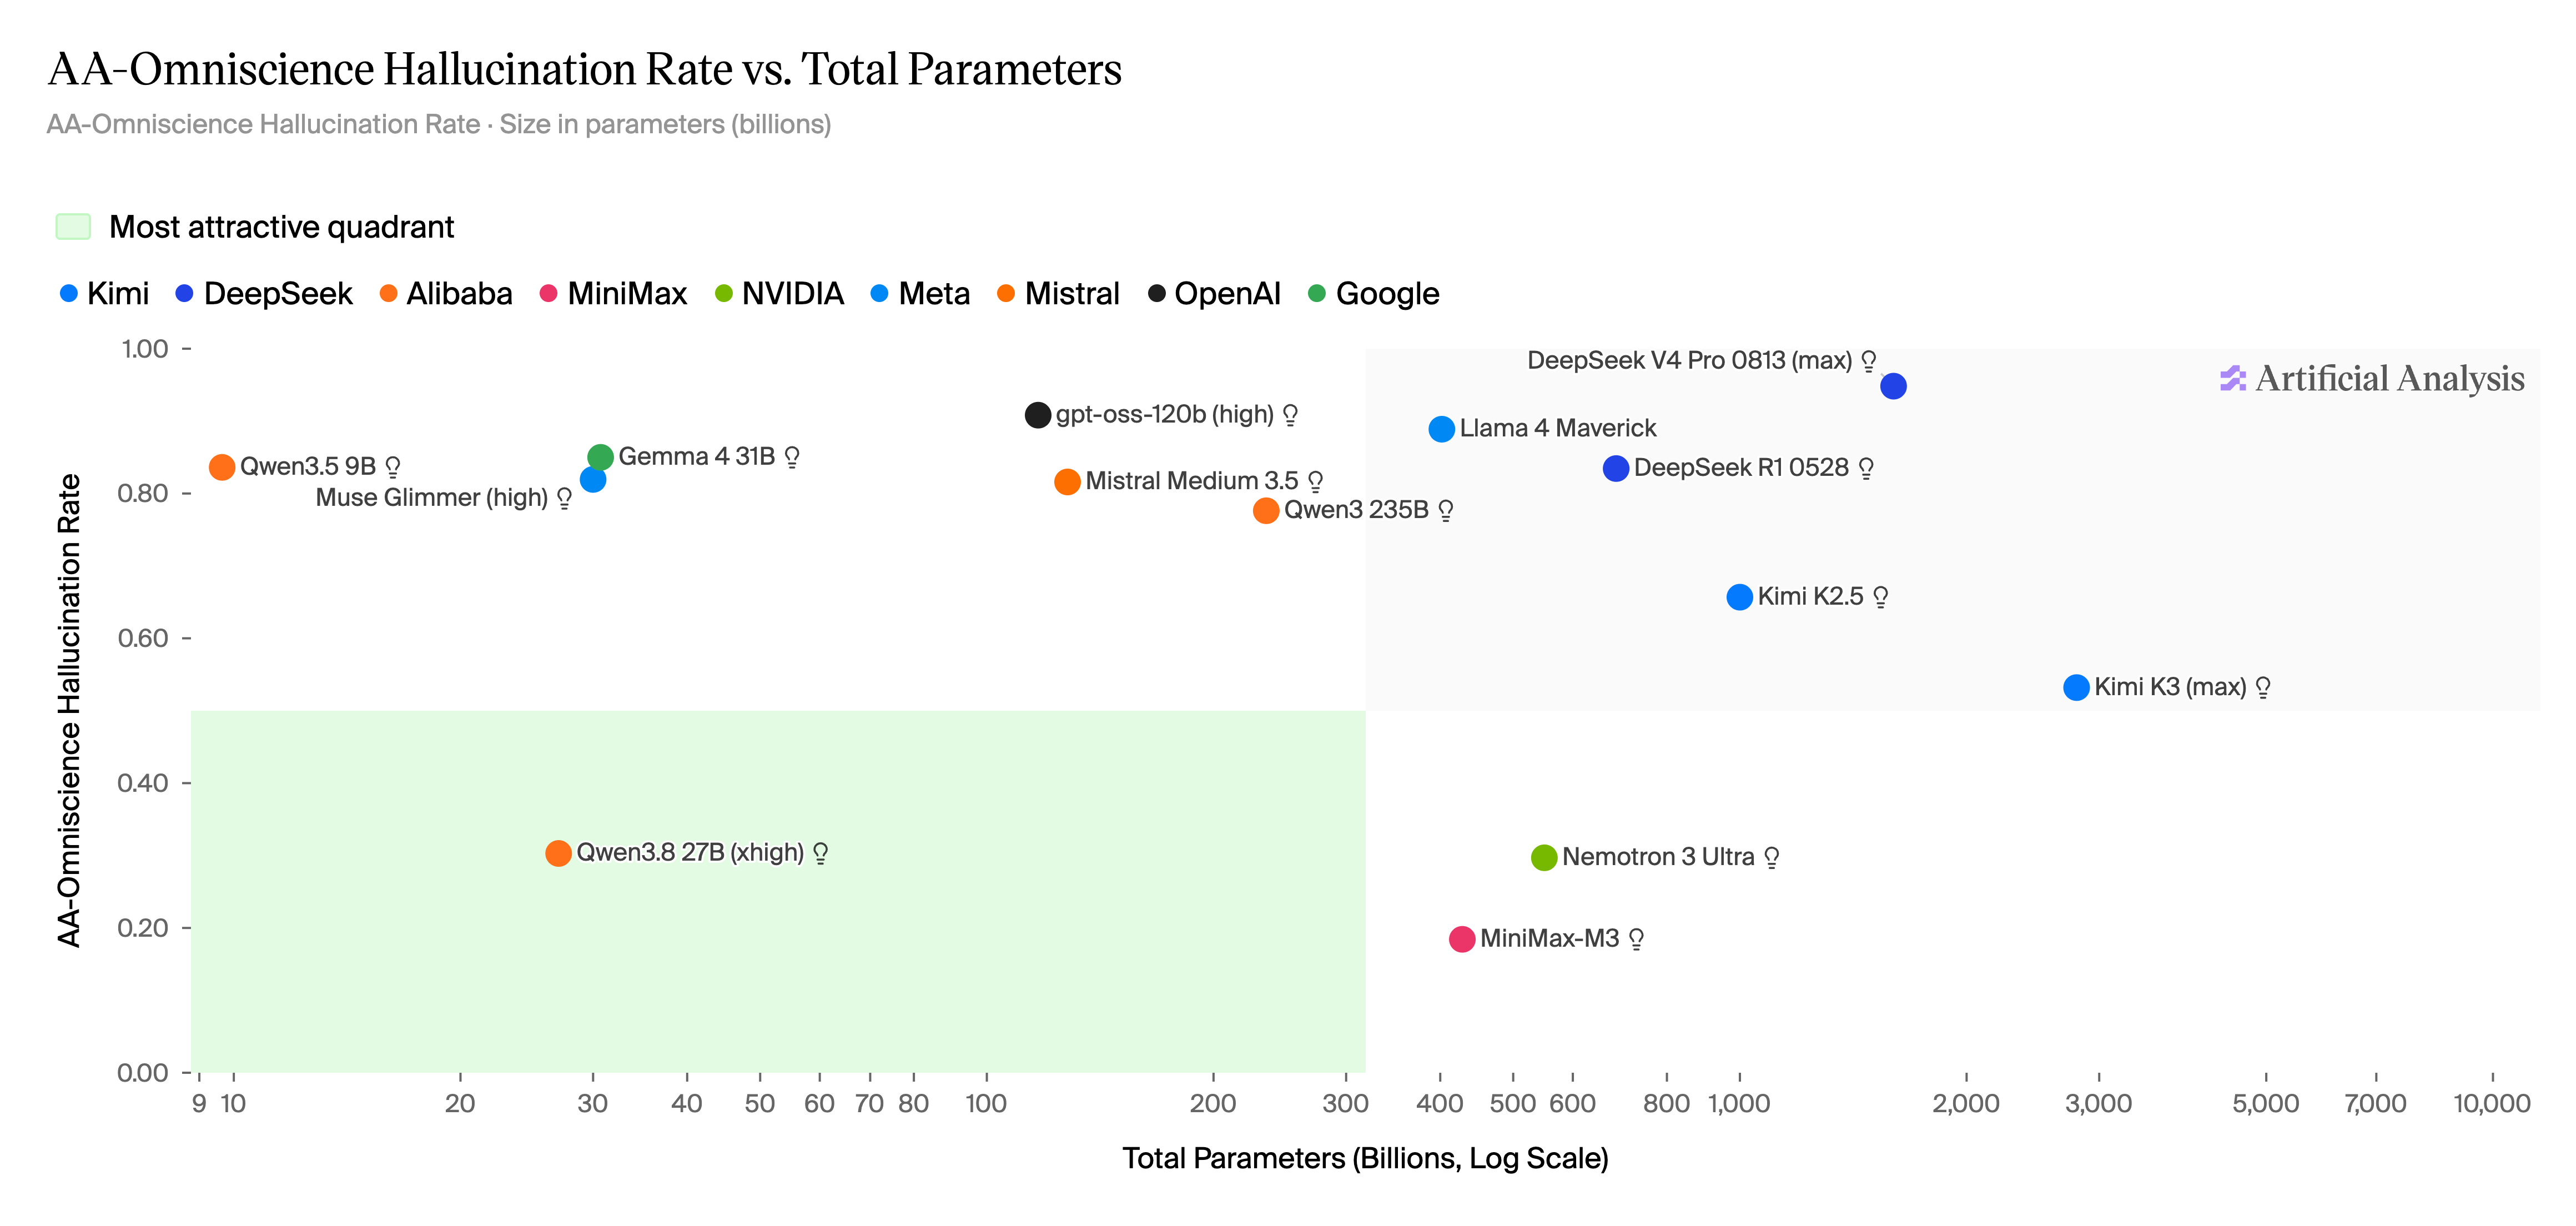
\includegraphics[width=0.98\linewidth]{figures/AA-Omniscience Hallucination Rate vs- Total Parameters (26 Aug '26) (1).png}}{\fbox{\parbox{0.90\linewidth}{\textbf{Source graphic not supplied.} Restore the original AA-Omniscience snapshot image from the source project. No measurements are reconstructed here.}}}
\par\smallskip
\IfFileExists{figures/AA-Omniscience Index - Score vs- Release Date (26 Aug '26).png}{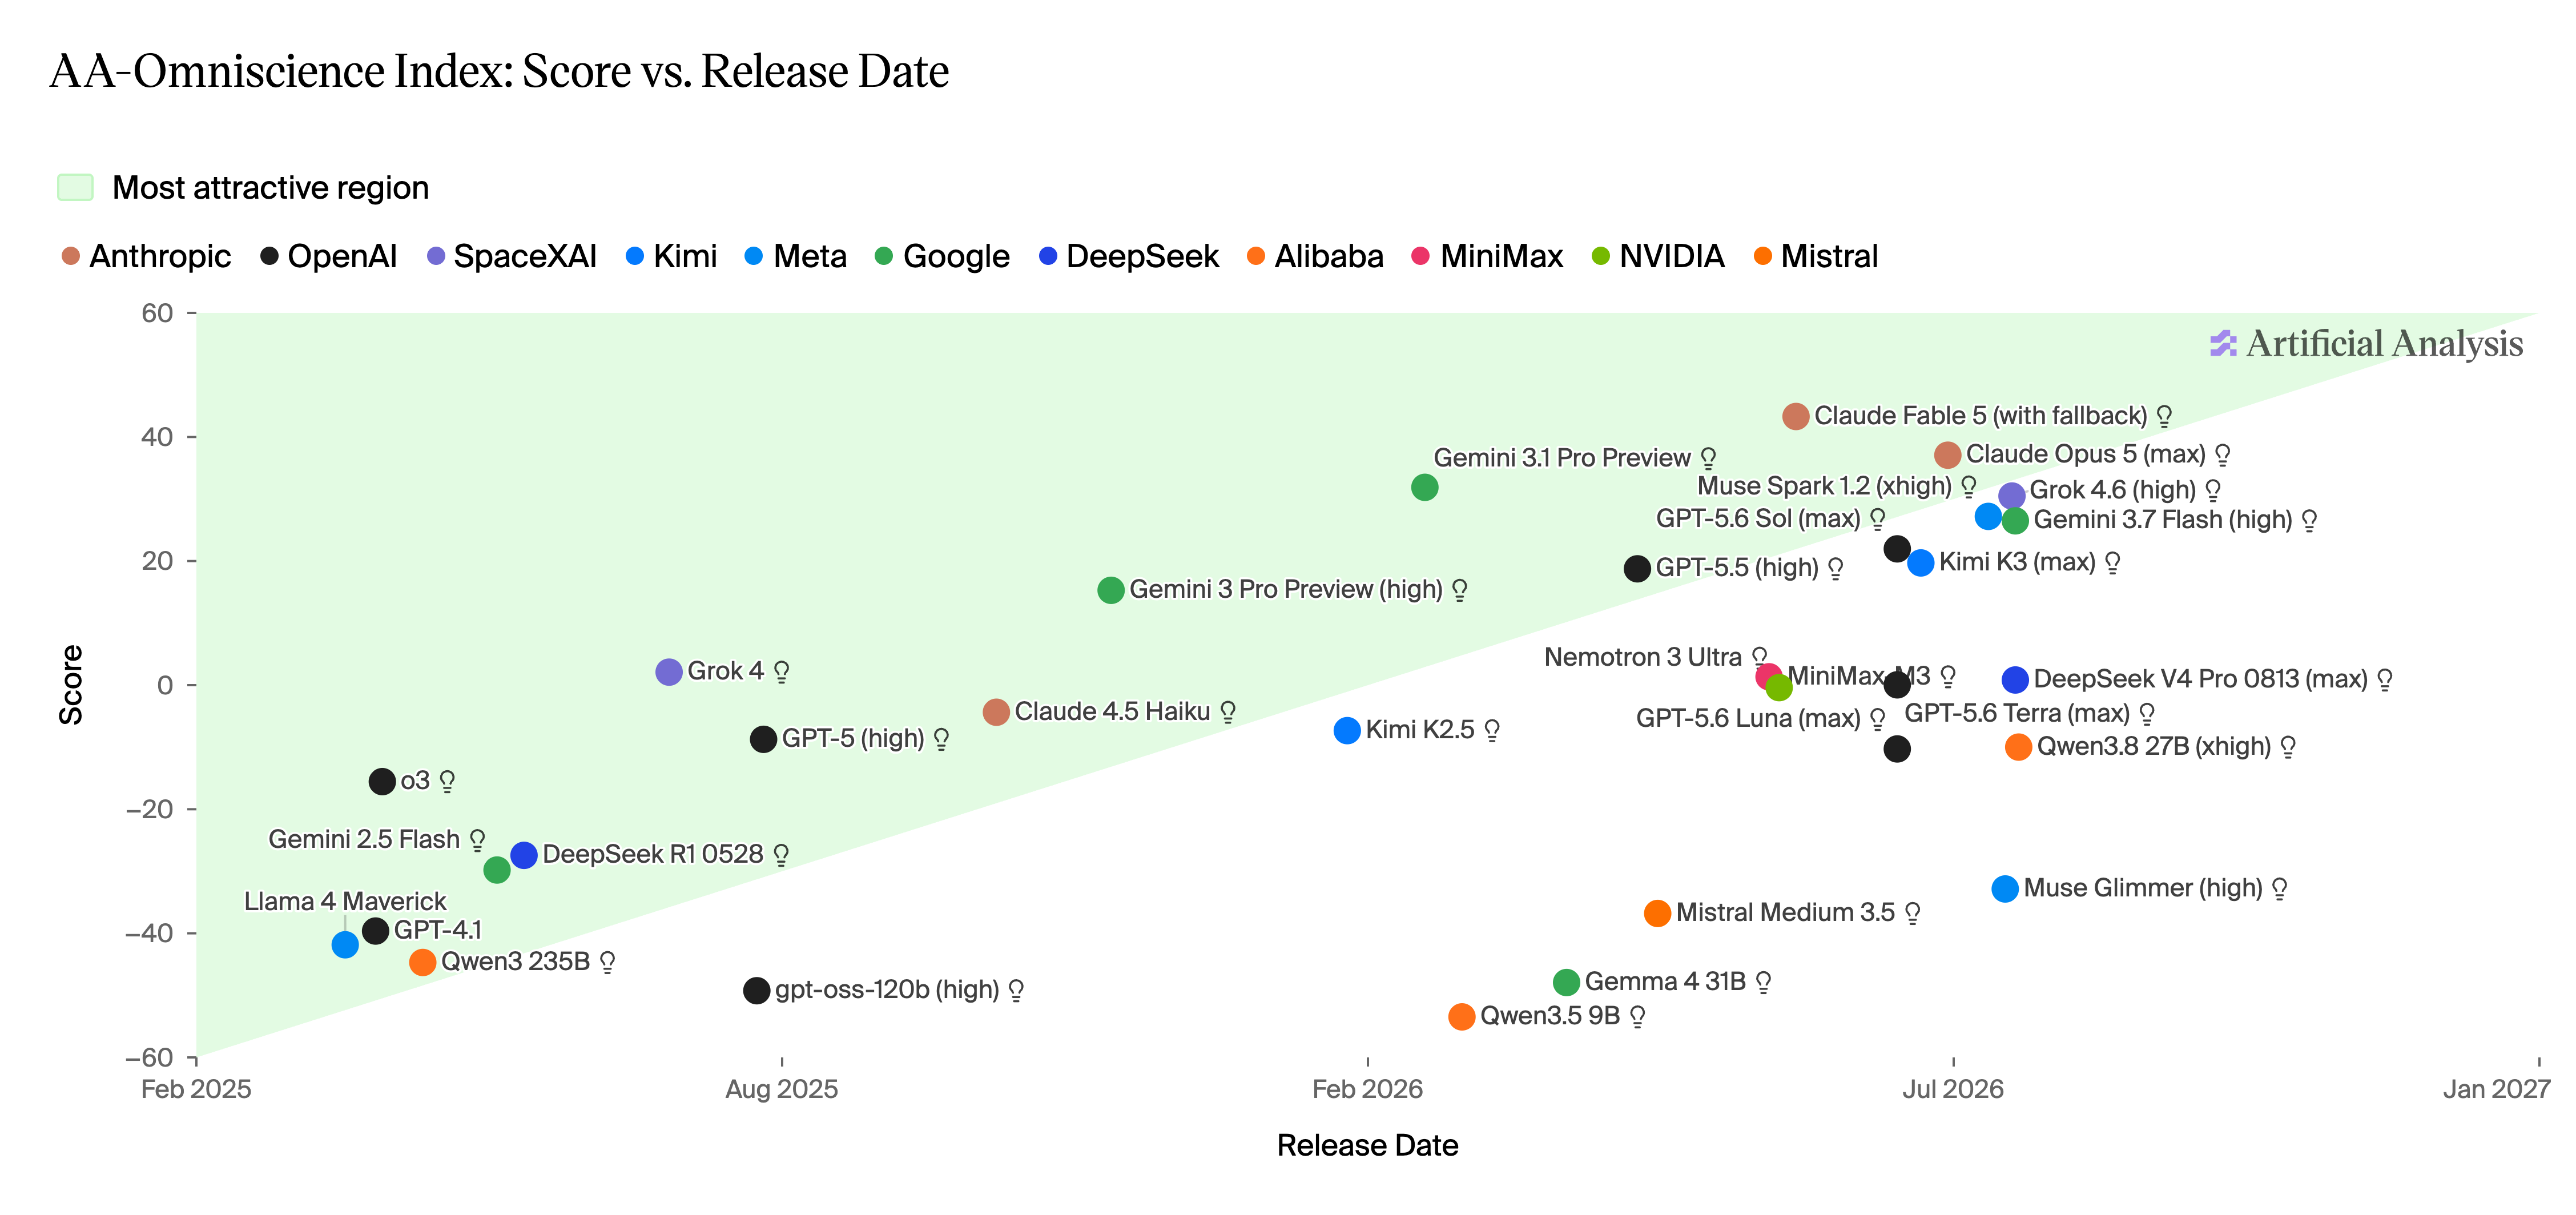
\includegraphics[width=0.98\linewidth]{figures/AA-Omniscience Index - Score vs- Release Date (26 Aug '26).png}}{\fbox{\parbox{0.90\linewidth}{\textbf{Source graphic not supplied.} Restore the original AA-Omniscience snapshot image from the source project. No measurements are reconstructed here.}}}
\caption{\textbf{AA-Omniscience leaderboard snapshot, August 26, 2026.}
Top: AA-Omniscience hallucination rate versus disclosed total parameters for
selected open-weight model configurations (lower is better; logarithmic
$x$-axis). Bottom: Omniscience Index versus release date for selected model
configurations (higher is better). The panels compare different models at one
date; they do not track one model family over time or isolate the effect of
model size. Source and graphics: Artificial Analysis
\citep{artificialanalysis_omniscience_leaderboard_2026}.}
\label{fig:aa-omniscience-snapshot}
\end{figure}

The plotted models differ in their developers, architecture, training,
post-training, and inference settings. The parameter panel includes only
models with a disclosed total parameter count. The release-date panel does
not hold these other choices fixed, and the leaderboard's grader and
methodology changed between the 2025 launch analysis and this snapshot.
The figures therefore cannot establish a causal relation between size or
release date and reliability, or prove that hallucination never decreases.
They provide descriptive context for Section~\ref{subsec:relative}, not
evidence that truth-contract evaluation works better than other methods.

\clearpage
\bibliography{references}

\end{document}
